\documentclass[letter, 10pt]{article}
\usepackage[utf8]{inputenc}
\usepackage[spanish]{babel}
\usepackage{amsfonts}
\usepackage{amsmath}
\usepackage[dvips]{graphicx}
\usepackage{subfigure}
\usepackage{url}
\usepackage{hyperref}
\usepackage{color}
\usepackage[top=3cm,bottom=3cm,left=3.5cm,right=3.5cm,footskip=1.5cm,headheight=1.5cm,headsep=.5cm,textheight=3cm]{geometry}
\usepackage{alltt}

\definecolor{red}{rgb}{1,0,0}
\definecolor{green}{rgb}{0,1,0}
\definecolor{blue}{rgb}{0,0,1}
\newcommand{\blue}{\textcolor{blue}}
\newcommand{\red}{\textcolor{red}}
\newcommand{\green}{\textcolor{green}}

\begin{document}
\bibliographystyle{plain}
\pagestyle{empty}



\title{
Taller de Modelos y Métodos Cuantitativos \\
\Large{
Proyecto Implementación Algoritmo \emph{``Clonal Selection''} para el \emph{``Car Sequencing Problem''}
}
}
\author{Cristián D. Maureira Fredes}
\date{\today}
\maketitle

\section{Introducción}
\label{sec:introduccion}
\frame
{
\frametitle{Introducción}
\begin{itemize}
	\item Motivación del problema.
	\item Sobre la técnica.
	\item Implementación inicial.
	\item Sintonización.
	\item \blue{Control}.
	\item Resultados.
\end{itemize}
}



\newpage
\section{Definición del Problema}
\label{sec:definicion}
%Descripción del problema, su complejidad, en que consiste, cuales son sus objetivos,
%restricciones, variantes más conocidas. 

El \emph{Car Sequencing Problem} es un problema de satisfacción de restricciones (CSP), posee la
característica de ser NP-duro~\footnote{
NP-duro es el conjunto de los problemas de decisión que contiene los problemas H
tales que todo problema L en NP puede ser transformado polinomialmente en H.
Esta clase puede ser descrita como conteniendo los problemas de decisión que son
al menos tan difíciles como un problema de NP.}
, además corresponde a un tipo de variación del problema NP-completo \emph{Job-Shop Scheduling}.%,
%pero con un uso de razonamiento automatizado, es decir, con un enfoque dedicado a estudiar y comprender
%diferentes características del razonamiento, permitiendo así construir programas que le den la posibilidad
%a los computadores para razonar en forma autónoma.
 
Siguiendo la misma idea, es válido señalar que el \emph{Car Sequencing Problem} es un tipo de problema de planificación
de tareas en una línea de ensamblaje de autos, donde cada uno es perteneciente a un clase de automóvil, debido al conjunto
de opciones y accesorios que posee (airo acondicionado, centralizado eléctrico, etc), y cada una de las opciones o
accesorios se instala en una planta distinta, por lo que el objetivo principal es el poder encontrar el orden en la
secuencia de los vehículos, preocupándonos de no exceder la capacidad de cada planta de ensamblaje y también cumplir con la demanda.

Por lo tanto, si realizamos una definición más formal de nuestro problema, podríamos decir lo siguiente:
Teniendo una lista de vehículos dada, cada uno con sus respectivas opciones requeridas,
necesitamos establecer un orden en la línea de ensamblaje, con el fin de que cada subsecuencia de $q$ vehículos
tengamos a lo más $p$ que requieren de una determinada opción. Es importante tener en consideración que los
valores de $p$ y $q$ están asociados a cada opción de los vehículos.

Con respecto a la información que el problema otorga, podemos decir que contamos con:
\begin{itemize}
	\item Cantidad de vehículos de cada tipo o clase a producir (demanda)
	\item Lista de las opciones con la cual se constituye cada tipo o clase de vehículo, la cual puede utilizar una representación
		booleana para saber si cierto tipo de automóvil posee o no una determinada opción.
	\item Capacidad de las plantas que se preocupan de instalar la determinada opción.
\end{itemize}

Nuestro objetivo principal es:
\begin{itemize}
	\item Encontrar un orden en nuestra secuencia, que sirva para minimizar el costo por cada restricción insatisfecha.
\end{itemize}

Con respecto a las restricciones, tenemos que:
\begin{itemize}
	\item En cada subsecuencia de los $q$ vehículos, a lo más pueden haber $p$ que requieran de la opción determinada.
		Donde $p$ y $q$ son valores asociados a cada opción.
	\item La capacidad de cada planta de ensamblaje no puede ser excedida, es decir, cumplir con la demanda de cada automóvil
		sin abusar de una planta determinada.
	\item Por cada tipo de auto, el numero de autos de ese tipo debe ser secuenciado, es decir, todos los automóviles de cada clase
		deben estar presente en una secuencia determinada.
\end{itemize}





\newpage
\subsection{Estado del arte problema}
\label{sec:estadoArte}
%Debe contener: técnicas usadas en su resolución (en general las que han sido mas
%efectivas a la fecha), mejores resultados, estrategias mas usadas en su resolución,
%representacion, movimientos, penalización, etc..


El \emph{Car Sequencing Problem}~\cite{parello} es presentado por primera vez en la \emph{Journal of Automated Reasoning},
del año 1986 en \emph{EEUU}, por \emph{B.D Parello}, \emph{W.C. Kabat} y \emph{L. Wos}, siendo una variación
del problema ya conocido en el área de la Inteligencia Artificial, como lo es el \emph{Job-Shop scheduling problem},
pero usando otro tipo de razonamiento, el \emph{Razonamiento automatiza}, de ésta manera logran enfocar su trabajo
en el problema que ocurre en las líneas de producción de automóviles.

Desde la publicación del presente problema hasta los últimos años, han aparecido en distintas conferencias a lo largo
del mundo, diferentes formas de atacar el problema, que nos llevan desde  ``programación lineal'', ``Evolutionary Approaches''
y ``Local search'' con sus variantes.

Las técnicas que han sido utilizadas hasta el momento, no han sido desarrolladas sólo por matemáticos, sino que por una amplia
gama de investigadores, que van desde científicos del área de la producción, física, biología y gestión.

No obstante, gracias a los avances que ha tenido el campo de la Inteligencia Artificial, han aparecido nuevas metodologías,
que se relacionan con otras áreas como lo son la computación evolutiva, genética,  redes neuronales, neurofisiología;
los cuales han realizado contribuciones importantes a los problemas que tienen que ver con la ``planificación'' (scheduling).
Lo anteriormente señalado afirma el hecho que los problemas relacionados con la ``planificación'' abarcan muchas áreas en el mundo,
y que los trabajos en dicha área no tienen que ver sólo con científicos computacionales.

A continuación se describen algunos de los métodos más importantes que han sido propuestos desde el año
en que el \emph{Car Sequencing Problem} fue dado a conocer en el mundo de la investigación científica.


\subsection{Acercamientos heurísticos}
Existen distintos acercamientos que se han propuesto, que tienen como objetivo principal
encontrar una solución óptima lo más rápido posible.
Los acercamientos descritos a continuación son \emph{búsqueda local (local search)},
\emph{greedy approach}, \emph{Ant colony Optimization} y por último, \emph{Algoritmos genéticos}

\subsubsection{Búsqueda Local (Local Search)}
La \emph{Búsqueda Local} puede ser utilizada en distintos problemas que se formulan
de una forma determinada para poder encontrar una solución que maximice un criterio alrededor de un número
de soluciones candidatas

Lo que hace la \emph{Búsqueda Local}, es moverse en su vecindario solución por solución en el espacio previamente establecido
de las soluciones candidatas, también conocido como espacio de búsqueda, hasta que una solución considerada \emph{óptima}
es encontrada ó se termina el plazo de tiempo para encontrar la solución, por otra parte, 
el vecindario va a estar definido netamente con respecto al modelamiento del problema.

Actualmente existen variadas aproximaciones propuestas sobre \emph{Búsqueda Local},
para resolver el presente problema.
La diferencia aquí, es que la mayoría de las propuestas son acercamientos más
genéricos, es decir, se han utilizado varios problemas para aplicar la propuesta
planteada y entre ellos se encuentra el problema en cuestión, como por ejemplo~\cite{DTWZ94}
que nos plantea una mejora en el sentido de una \emph{Estrategia de Búsqueda}, considerando
el conflicto mínimo con respecto a la heurística \emph{hill-climbing}~\footnote{
Técnica de optimización matemática, puede ser usada para resolver problemas con muchas soluciones.
Consiste en escoger una solución aleatoria (potencialmente no óptima) y comienza a
realizar pequeños cambios a dicha solución en cada iteración, en cada momento se va mejorando un poco más.
}
y ha propuesto un escape con respecto a los mínimos locales incrementando el peso de las
restricciones que no se cumplen.

Por otra parte existen otras propuestas que se han enfocado netamente en resolver éste problema,
como es el caso de ~\cite{PG02}, que considera los algoritmos de \emph{Búsqueda local}
que se basan en una representación de una permutación y la evaluación de las restricciones que no se
cumplen utilizando funciones de penalización.

De la misma forma tenemos el caso de lo que plantea Gottlieb et al. en \cite{GPS03}, quien se refiere
a una parte en especial de nuestro problema, la construcción de la secuencia inicial, por lo tanto
sabemos que en la mayoría de los casos, la secuencia inicial de vehículos, de donde parte la
\emph{Búsqueda Local}, es una permutación aleatoria de un conjunto de vehículos para comenzar
a ensamblarlos, sin embargo la propuesta nos señala el construir ésta secuencia inicial en una forma
\emph{Voraz (Greedy)}~\footnote{
se refiere a a realizar una elección del siguiente elemento considerando una función heurística de optimización,
con la esperanza de llegar a una solución general óptima.
}
, lo que queda claramente demostrado en dicha publicación,
debido a las grandes mejoras en el proceso de solución.

\subsubsection{Acercamiento Voraz (Greedy approaches)}
Teniendo en consideración el \emph{Car Sequencing Problem}, podemos construir una secuencia
en una forma \emph{Voraz (Greedy)}, eligiendo el siguiente vehículo de la secuencia
considerando una función heurística de optimización.
El primero acercamiento utilizando \emph{Greedy} fue propuesto por
Hindi and Ploszaski en 1994~\cite{HP94}. Volviendo al procedimiento anteriormente descrito, la idea
central que nos plantea Gottlieb et al. en \cite{GPS03}. Claramente, ahora la elección que podemos
realizar en cada paso de nuestro algoritmo, debe ser la más óptima, en otras palabras,
elegir el vehículo que posea el menor número de restricciones no satisfechas.

Matemáticamente hablando, podríamos decir lo siguiente:
Dado una secuencia parcial $\pi$, el siguiente vehículo es seleccionado entre los vehículos $c_j$
que minimice la siguiente función,
$$newViolations(\pi, c_j) = \sum_{o_{i}\in O}r(c_j,o_i)\cdot violation(lastCars(\pi\cdot <c_j>,q(o_i)),o_i)$$
donde $o_j$ es una opción del vehículo $c_j$ y donde $lastCars(\pi',k)$ es la secuencia compuesta de los
últimos $k$ vehículos de $\pi'$, si $|\pi'| \geq k$, en otro caso $lastCars(\pi' , k) = \pi')$.

El problema acá, es que por lo general, el conjunto de vehículos seleccionados que minimizan la función
$newViolations$, contiene más de un auto, por lo tanto acá viene otra decisión importante. ¿Cuál de esos
autos elegimos?, por lo que Gottlieb et al.~\cite{GPS03} nos señala que es necesario utilizar otra técnica heurística para 
romper dicha incertidumbre, de la misma forma propone 6 heurísticas distintas. La heurística que presente
un mejor desempeño es llamada \emph{``dynamic sum of utilization rates''}, la cual consta en que en cada paso
añadimos el vehículo que maximiza la suma de las tasas de uso de opciones necesarias, estas tasas de uso se actualizan
dinámicamente cada vez que añadimos un nuevo auto al final de la secuencia.

\subsubsection{Ant Colony Optimization (ACO)}
El algoritmo \emph{Ant Colony Optimization (ACO)}, tal como es descrito en \cite{DS05},
toma su inspiración en el comportamiento de ciertas especies de hormigas. La idea central
es notar que las hormigas depositan en el suelo una feromona, con el objetivo de marcar
un camino favorable para que los otros miembros de su colonia puedan seguirlo. Por lo tanto
\emph{ACO} busca aplicar un mecanismo similar para resolver problemas de optimización.

En otras palabras, \emph{ACO} es una forma de modelar cierto problema de tal forma
que busquemos siempre el camino con mínimo costo en un grafo determinado, y por supuesto,
utilizar \emph{hormigas artificiales} para buscar los caminos que más nos pueden favorecer.


El primer algoritmo de \emph{ACO} fue propuesto por Christine Solnon~\cite{Sol00},
y se trata de resolver un problema de satisfacción de restricciones de permutación~\footnote{
El objetivo principal es poder encontrar la permutación de $n$ valores conocidos,
para asignarlos a $n$ variables, bajo ciertas restricciones.
},
utilizando el concepto de \emph{hormigas artificiales}. Principalmente está diseñado
para resolver un problema general de combinatoria.

En enfoque que entrega el trabajo previamente señalado~\cite{Sol00} con respecto
al \emph{Car Sequencing Problem} es el siguiente:
Recordando nuestro problema principal, sabemos que consiste
en realizar la óptima planificación de los vehículos en una línea de ensamblaje,
donde tenemos $n$ vehículos para producir, que están agrupados en $k$ tipos
de autos~\footnote{
Cada conjunto de autos de un mismo tipo tienen las mismas opciones
}, y sabemos también que cada opción $i$ está asociada con una restricción de capacidad
representada por una tasa $p_i/q_i$, que especifica que para cualquier secuencia
de $q_i$ autos consecutivos en le línea de ensamblaje, tenemos al menos $p_i$ vehículos
que requieren dicha opción.
Finalmente el objetivo será encontrar una permutación de $n$ vehículos que satisfacen
todas las restricciones de capacidad, tomando en consideración que nuestra feromona
se pondrá sobre las parejas de los vehículos consecutivos con el fin de aprender
las sub-secuencias de vehículos más prometedoras (óptimas).

No conforme con el desempeño mostrado en el trabajo anterior, Gottlieb et al.~\cite{GPS03}
proponen un nuevo algoritmo que introduce tres nuevas mejoras:
\begin{itemize}
	\item Se utiliza una estrategia elitista, por lo que la feromona es usada para romper el lazo entre los mejores vehículos solamente.
	\item Se integran mejoras del trabajo ~\cite{Stu}, para favorecer la exploración.
	\item Se usan funciones heurísticas de tipo \emph{voraz (greedy)} para guiar las hormigas.
\end{itemize}
Con las mejoras anteriormente planteadas se logra obtener un resultado mucho más óptimo computacionalmente.

\subsubsection{Algoritmos Genéticos (Genetic Algorithms)}
Los \emph{Algoritmos Genéticos} son una técnica computacional que tienen como objetivo principal,
el encontrar una solución exacta o aproximada en problemas de optimización y búsqueda.

En el trabajo de Warwick y Tsang~\cite{WT95} se propone un algoritmo genético especialmente
para resolver el \emph{Car Sequencing Problem} que se diferencia de los algoritmos genéticos
tradicionales pues ingresa ciertas características especiales como el \emph{elitismo}~\footnote{
proceso de seleccionar mejores individuos, seleccionándolos con el fin de obtener una mejor solución
}, plantillas adaptativas de \emph{crossover}~\footnote{
operador genético utilizado para variar la programación de uno o varios cromosomas, de una generación  a otra.
}, \emph{hill-climbing}, entre otras.

El acercamiento que nos ofrece éste mecanismo tiene su origen en una especie de inspiración
de la evolución natural y trata de introducción computacionalmente los conceptos de \emph{cross over},
\emph{mutación}, y tomar las secuencias de nuestros problemas, como una \emph{población}.

Por lo tanto, el procedimiento que realiza es que por cada \emph{generación}, las secuencias
que son seleccionadas se combinan gracias al operador \emph{cross over}, y se obtiene lo
que se denomina \emph{descendencia} que puede que no satisfaga la restricción global,
pero se va reparando en cada iteración y luego se le aplica \emph{hill-climbing} mediante
una función de intercambio.

Lamentablemente el procedimiento anteriormente descrito es bueno para resolver sólo,
versiones no tan complejas del \emph{Car Sequencing Problem}.
Debido a lo anterior Cheng et al. \cite{CLP+99} propone un algoritmo para resolver un
problema práctico, es decir, más realista, con un grado mayor de complejidad.
Cheng et al. \cite{CLP+99} proponen un operador llamado \emph{cross-switching},
que genera una descendencia intercambiando los vehículos que aparecen de forma aleatoria
en la primera secuencia del problema.

\subsubsection{Movimientos}

A continuación se explican brevemente algunos movimientos conocidos que definen el vecindario de 
una solución, y que de la misma forma, es válido para cualquier acercamiento anteriormente
mencionado.
\begin{enumerate}
	\item \emph{shift}: Puede realizarse con repecto a la izquierda o derecha, y avanzando una cantidad determinada de espacios,
		es decir, tomamos nuestra secuencia numérica, y la movemos para alguno de los dos lados. El hecho de que sea a la izquierda
		o derecha y la cantidad de espacios que se mueve, se puede elegir de manera aleatoria.

		\emph{e.g:} 1 0 1 0 0 1, aplicamos shift-right 2 veces y nos queda 0 1 1 0 1 0.
	\item \emph{swap}: Este movimiento es muy utilizado, pues ha demostrado tener alta eficiencia al momento de buscar
		nuevas soluciones, sin romper restricciones. Consiste en tomar dos elementos de nuestra secuencia, que pueden ser escogido
		de forma aleatoria, e intercambiarlos
		de lugar.

		\emph{e.g:} 1 0 1 0 0 1, aplicamos swap(1,5) y nos queda 1 1 1 0 0 0.
	\item \emph{bit-flip}: Éste movimiento consiste en cambiar el valor de un \emph{bit} de nuestra secuencia numérica.
			Sólo es válida para representaciones binarias (0 o 1). Para escoger que elemento cambiamos, lo podemos hacer de una forma
			aleatoria.
		
		\emph{e.g:} 1 0 1 0 0 1, aplicamios bit-flip(3) y nos queda 1 0 1 1 0 1.
	\item \emph{Cruzamiento en un punto (Single Point Crossover)}: La presente técnica consiste en tener dos individuos,
		elegir un punto al azar dentro de la secuencia y cruzarlos, intercambiando su material. También existen otras variaciones
		de éste movimiento, donde se elige más de un punto para intercambiar el material de los padres.

		\emph{e.g:} 1 0 1 1 y 1 1 0 1, elegimos el punto 2 y nos quedan dos hijos de la forma, 1 0 0 1 y 1 1 1 1.
				
	\item \emph{Técnica incompleta}: Es posible utilizar una misma técnica incompleta como \emph{movimiento} para poder generar
		el vecindario determinado, lo cual en la mayoría de las veces, produce secuencias mucho mejor, pero toma mucho más tiempo
		que los movimientos descritos anteriormente.
\end{enumerate}

\subsection{Acercamientos completos}
\subsubsection{Integer Lineal Programming}
En el trabajo de Grevel et al.~\cite{4} se propone un acercamiento utilizando
\emph{Programación Lineal Entera}, ILP por sus siglas en inglés,  para una variante
del problema famoso de \emph{Car sequencing problem} pero del concurso ROADEF,
donde ahí se establece condiciones extras relacionadas a la pintura de los vehículos,
que éste modelamiento no posee.

Grevel et al.~\cite{4} también nos da a entender que se puede resolver el problema
de una manera común, con ésto nos referimos a usando un simple \emph{benchmark}
con aproximadamente unos $200$ vehículos y $5$ componentes, probando así
lo óptimo que es el método, con un tiempo de respuesta razonable.
La idea principal que posee éste mecanismo o modelamiento, es poder aplicarla a un
grupo de vehículos con la misma configuración, con respecto a las opciones,
evitando así simetrías entre ellos.

Existe otra aproximación relacionada con ILP, presentada por Prandtstetter et al.~\cite{12}
que es análoga a la formulación realizada por Gravel et al., clasificando los vehículos
que tienen la misma configuración en grupos, gracias a ésto el tamaño de alguna instancia
del problema que sea propuesto, está restringido a lo más $300$ vehículos con aproximadamente
unos $8$ componentes.

\subsubsection{Ramificación y Poda (Branch-and-bound method)}

El presente método es una variación del algoritmo \emph{Backtracking}~\footnote{
la idea del algoritmo se asemeja a un recorrido en profundidad dentro de un grafo dirigido.
}
, pero con bastantes mejoras.
Por lo general, la idea es interpretar el problema como un árbol de soluciones,
en el cual las ramas van a ser caminos para una posible solución, pero posterior a la solución
actual (rama actual).
La idea central del presente método es que se encarga de encontrar las ramas que no poseen
una solución óptima en comparación al resto y las \emph{poda} para no utilizar el tiempo
de búsqueda en alguna rama que no sirva.

En el trabajo de Drexl et al.~\cite{DKM06}, se propone utilizar la misma técnica anteriormente
descrita.

Primeramente es un poco complicado por imaginarse el problema atacado del punto de vista
del \emph{Branch-and-bound}, debido a que se toma como un problema de grafos, pero lo que
Drexl et al.~\cite{DKM06} establece es que el método está basado en un esquema de ramificación
\emph{(branching)} original, que utiliza el concepto de \emph{Car sequencing state}, 
refiriéndose así a que cada \emph{Car sequencing state} está asociado a cada nodo del árbol
que podemos construir para resolver el presente problema.

Para comenzar el \emph{branching}, es necesario construir una secuencia $\delta$
asignando cada periodo $t\in {1,...,V}$ a una copia de una variante $v$, realizando ésto
se puede manipular la secuencia $\delta$ de la forma:
$$\delta : \{1,...,T\}\rightarrow\{1,...,V\}\cup\{0\}$$~\footnote{
Se agrega el $0$ para evitar las secuencias parciales, asumiendo que ningún periodo no asignado
está siendo proyectada a una variante vacía. Ésto simplifica las definiciones, sin restringirlas.
}, con
\begin{itemize}
	\item $T:$ volumen total de producción (periodos, ciclos), i.e $T=\sum\limits_{v=1}^{V}D(v)$, índice $t$
	\item $V:$ número de variantes, índice $v$
\end{itemize}

La secuencia $\delta$ induce una matriz $O\times T$ que llamaremos $M$,
la cual está representando los periodos de la planificación de T,
y cada file de $M$ incide con una opción $j$
, con
\begin{itemize}
	\item $O:$ número de opciones, índice $j$.
\end{itemize}

La interpretación de la matriz de la matriz $M$ se define a continuación:\\

$m_{j,t} = \left\{ \begin{array}{l}
\ \ 1,\ \text{si la opción}\ j\ \text{es planificada en el periodo}\ t,\ \text{respetando la restricción}\ H_{j}:H_{j}\\
\ \ 0,\ \text{si la opción}\ j\ \text{puede ser planificada en el periodo}\ t\\
-1,\ \text{si la opción}\ j\ \text{no es planificada en el periodo}\ t\text{, si es planificada puede violar}\\
\ \ \ \ \ \text{la restricción}\ H_{j}:H_{j}\\
\end{array} \right.$

\subsubsection{Constraint Programming}

El método \emph{Constraint Programming} es una herramienta genérica para poder resolver problemas
del tipo \emph{Constraint  Satisfaction Problem (CSP)}~\footnote{No confundir con Car Sequencing Problem},
por lo tanto cualquier problema de \emph{scheduling} puede ser resuelto mediante ésta forma,
ya que conjunto de restricciones que debemos satisfacer son una relación entre varias variables desconocidas,
y otras variables conocidas~\cite{Tsa93}.

%
Por lo general para obtener una solución óptima, se suelen combinar técnicas heurísticas,
y otras para deducir restricciones derivadas, como la clausura.
Como es el caso de Alfonso y Barber~\cite{esp1}, el cual utiliza un método primero de \emph{constraint-posting},
que significa ir adicionando sucesivamente las restricciones y en cada paso realizar el proceso de clausura,
en otras palabras incorporan el proceso de clausura que determina el conjunto de las restricciones que pueden
impedir  en las que ya se han asertado correctamente.

Dejando de lado el trabajo anteriormente mencionado, el método de \emph{Constraing Programming} permite la definición
y aplicación de nuevas técnicas de heurística, permitiendo así limitar el número de disyunciones
del conjunto de las restricciones y además permiten dirigir mejor el proceso de búsqueda.

\subsection{Acercamientos híbridos}

Cuando hablamos de acercamiento híbrido, nos referimos a poder combinar las ventajas de varios
métodos de optimización en un sólo algoritmo.
Anteriormente vimos que en muchos casos, existe inclusive una \emph{recomendación} para buscar
una heurística determinada complementando a un método y encontrar una solución óptima.


Tomando las palabras del estudio realizado por E.G Talbi~\cite{talbi} los algoritmos híbridos
se han aplicado satisfactoriamente a variados problemas de optimización combinatorial, como el problema
del \emph{vendedor-viajero} o simplemente problemas del mundo real.


Siguiendo las palabras de Blum, Roli y Alba en ~\cite{blum} podemos aseverar que ésta clase de acercamientos,
combinando metaheurísticas basadas en  poblaciones con alguna solución metaheurística simple, podemos llegar
a la conclusión de que es el mejor camino para poder mejorar la calidad de las soluciones que encontramos
en cualquier problema de optimización.

\subsubsection{Hybrid Integrative Evolutionary Approaches}
En el trabajo de Zinflou et al. \cite{HYB1} se presentan tres acercamientos para poder
resolver el presente problema. Los acercamientos están basados en esencia en algoritmos evolutivos
que incorporan operadores de heurística como los son los \emph{crossover operators} usando
un modelo simple, es decir basado en  Programación Lineal Entera.

La diferencia que existe entre dos de las aplicaciones de \emph{crossover} combinadas nos muestra que es posible
obtener valores competitivos, dignos de ofrecer como alternativa a los métodos anteriormente nombrado, debido
a la calidad de la solución.

Finalmente podemos darnos cuenta que la experiencia numérica de la formulación de éste método, muestra una diferencia
notoria en el tiempo de ejecución, algoritmicamente hablando.
Las diferencias indican que puede ser posible de obtener mejoras en la implementación de métodos híbridos para 
poder obtener una comparación más competitiva. Dichas mejoras significan poder involucrar al desarrollo de nuestro
algoritmos un enfoque de \emph{Grid computing} u otras técnicas de \emph{high performance computing technologies}.


\newpage
\section{Descripción de la Técnica}
\label{sec:tecnica}
%Origen de la técnica, descripción de la metáfora, componentes, modelos que existen etc.
\subsection{Origen biológico}

El principio de selección clonal es un modelo que explica la forma en la cual el sistema inmune
responde a una determinada infección y como algunos tipos de linfocitos T y B son seleccionados
para destruir un determinado antígeno que está invadiendo el cuerpo del sujeto.

Fue propuesto por el virólogo australiano, Sir Frank Macfarlane Burnet en el año 1959,
con un trabajo titulado \emph{``The clonal selection theory of acquired immunity''}.

Existen cuatro postulados fundamentales en la hipótesis de la selección clonal, los cuales son detallados más adelante:
\begin{enumerate}
	\item Cada linfocito soporta un solo tipo de receptor con una única especificación.
	\item La ocupación del receptor es requerida para la activación de la célula.
	\item Las células efectoras diferenciadas derivadas desde un linfocito activado soportarán receptores de una especificación idéntica al de la célula padre.
	\item Aquellos linfocitos que soportan receptores para moléculas propias serán eliminados en una etapa temprana.
\end{enumerate}

%[[
%The clonal selection theory is proposed by Burnet in 1978, the main features of which are summarized as following [8]:
%(1) The new cells are copies of their parents (clone) subjected to a mutation mechanism with high rates (somatic hyper-mutation);
%(2) Elimination of newly differentiated lymphocytes carrying self-reactive receptors;
%(3) Proliferation and differentiation on contact of mature cells with antigens;
%(4) The persistence of forbidden clones, resistant to early elimination by self-antigens, as the basis of autoimmune diseases.
%]]

De acuerdo a la teoría propuesta por Burnet, el repertorio del sistema inmune se somete a un mecanismo de selección durante el tiempo de vida de un individuo.
La teoría establece que al unirse con un antígeno adecuado, se produce la activación de los linfocitos.
Una vez activado, los clones de los linfocitos son producidos con receptores idénticos a los linfocitos originales que encontraron el antígeno.
Así ocurre una expansión clonal de los linfocitos originales.
Esto asegura que solo los linfocitos específicos que se han activado gracias a un antígeno sean producidos en grandes cantidades.
La teoría de la selección clonal también establece que cualquier linfocito que tenga receptores de antígenos de moléculas propias del organismo
debe ser eliminada durante el desarrollo de los linfocitos.
Esto asegura que solo los antígenos de un patógeno pueden causar que un linfocito se clone y se expanda y así generar una respuesta inmune adaptativa a
agentes externos.
Durante la expansión clonal de linfocitos B, el promedio de la afinidad entre los anticuerpos aumenta para el antígeno que desencadena la expansión clonal.
Este fenómeno se llama maduración de la afinidad, y es responsable de el hecho de que en una posterior exposición al antígeno, la respuesta inmune es más eficaz debido a los anticuerpos con una mayor afinidad por el antígeno.
La maduración de la afinidad es causada por una hiper-mutación somática y un mecanismo de selección que ocurre durante la expansión clonal de linfocitos B.
La hiper-mutación somática altera la especificación de los anticuerpos, introduciendo cambios aleatorios a los genes que lo forman.
\begin{figure}[h!]
\begin{center}
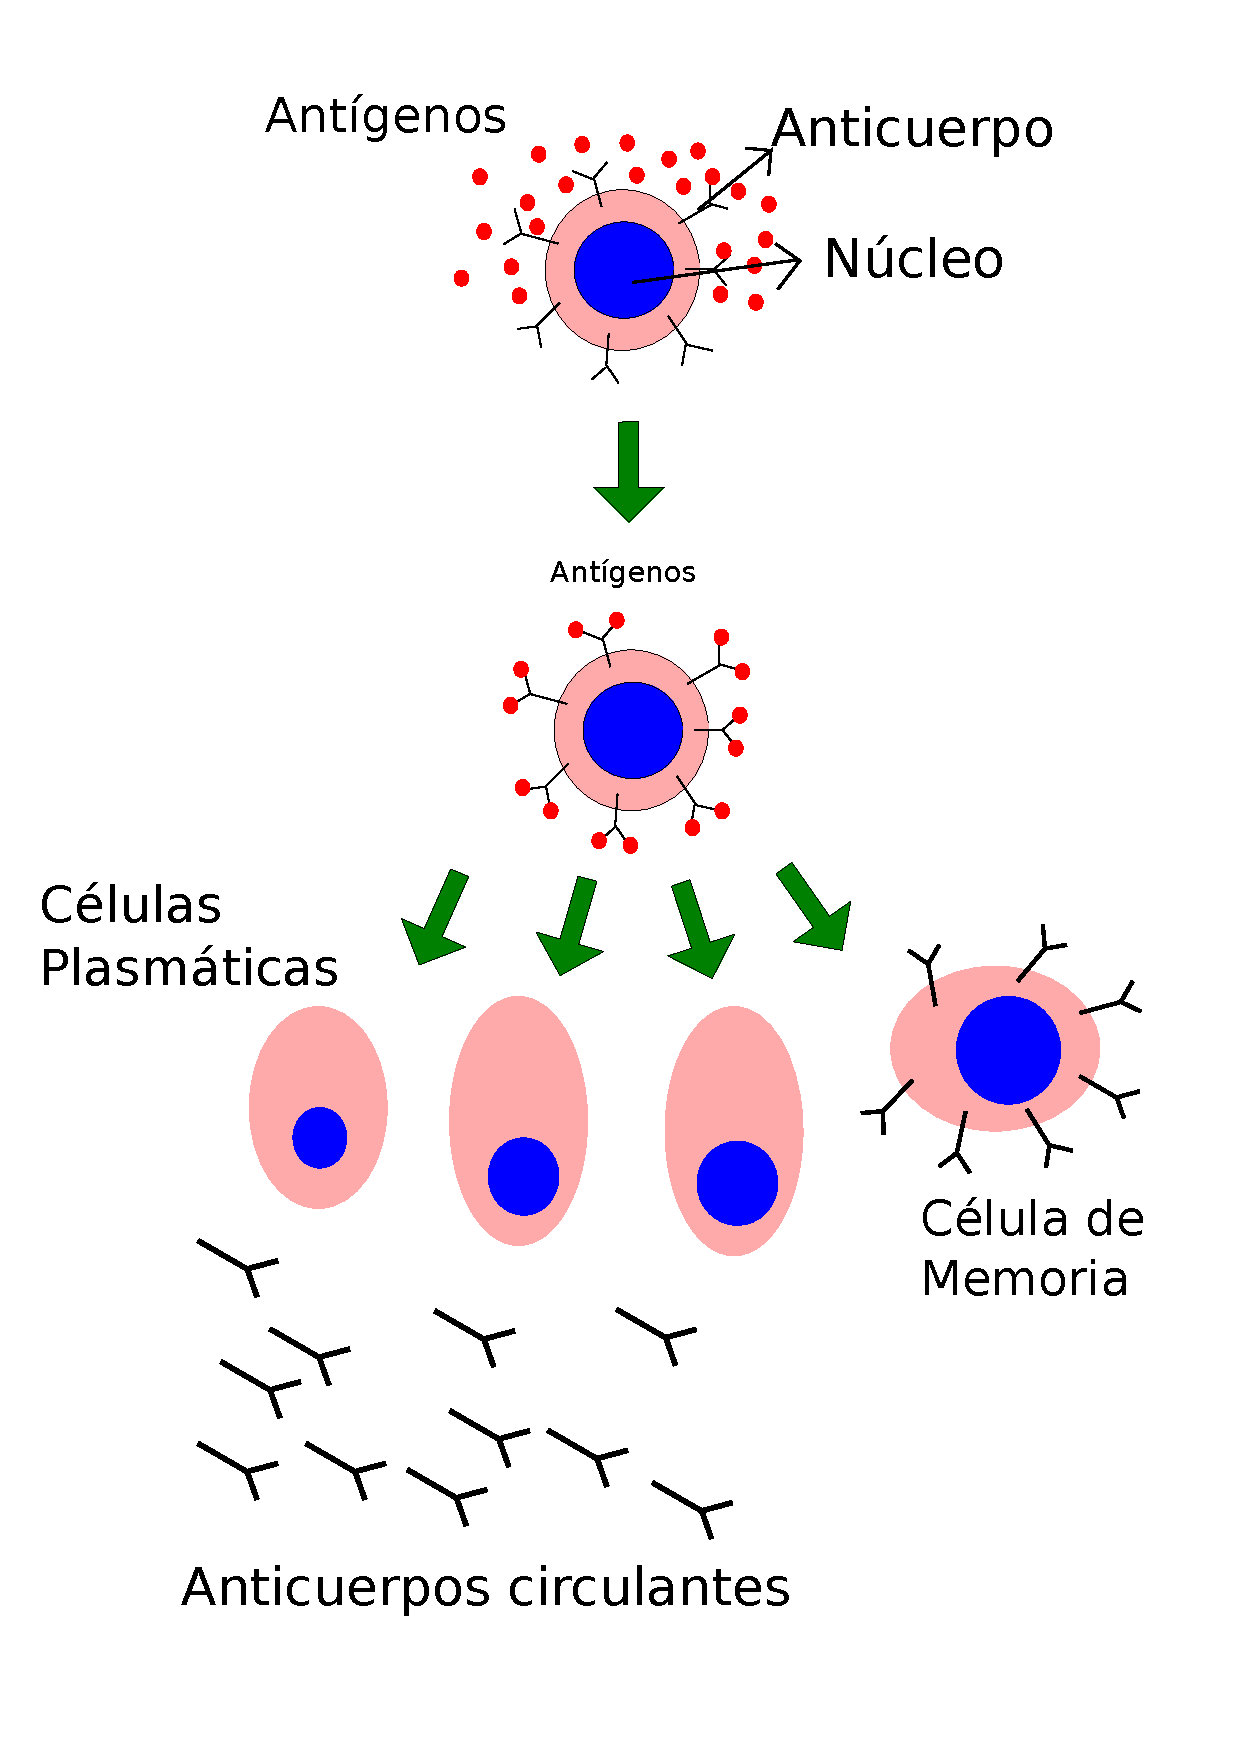
\includegraphics[width=0.5\textwidth]{img/clonalSelection.pdf}
\end{center}
\caption{Ejemplo de una selección clonal de linfocitos}
\label{fig:clonalSelection}
\end{figure}

Se señala la descripción de la figura~\ref{fig:clonalSelection} se detalla a continuación:

La teoría de la selección clonal de los anticuerpos indica que un linfocito B immaduro
se activa frente a la exposición de los antígenos, su posterior diferenciación en células
plasmáticas que sintetizan anticuerpos específicos en contra del antígeno y células de memoria.


\subsection{Algoritmo de la Selección Clonal}

Siguiendo el principio de selección clonal y el proceso de maduración de la afinidad, postulado por De Castro~\cite{decastro} se puede describir el algoritmo de selección clonal de la siguiente forma:
\begin{figure}[h!]
\begin{center}
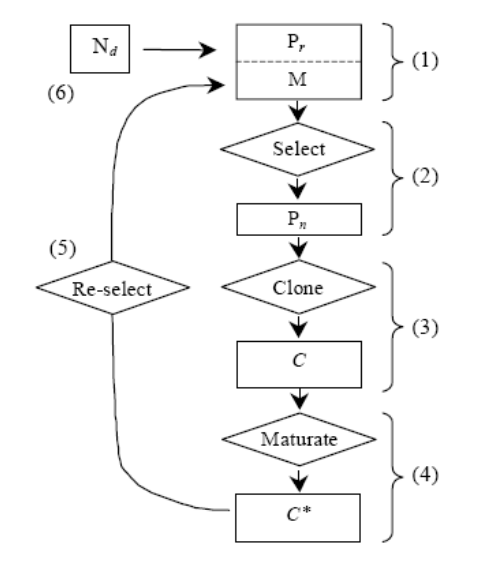
\includegraphics[width=0.5\textwidth]{img/algoritmo}
\end{center}
\caption{Diagrama del algoritmo de la selección clonal}
\label{fig:algoritmo}
\end{figure}

Siendo la explicación de los pasos de la figura~\ref{fig:algoritmo} la siguiente:
\begin{enumerate}
    \item Generar un conjunto (P) de soluciones candidatas, compuesto de células de memoria (M) añadidas a la población restante (Pr), teniendo entonces $P = Pr + M$
    \item Determinar los $n$ mejores individuos (Pn) de la población (P), basado en una medida de afinidad.
    \item Clonar (reproducir) estos $n$ mejores individuos de la población proporcional a su fitness, dando origen a una población temporal de clones (C).
    \item Someter la población de clones a un esquema de hiper-mutación (inversamente proporcional a la afinidad del anticuerpo). Una población de anticuerpos maduros es generada (C*).
    \item Seleccionar nuevamente los mejores individuos de (C*) para componer el conjunto de memoria. (Algunos reemplazos desde (C*) a (P), debido a la mejora)
    \item Reemplazar los $d$ anticuerpos con menor afinidad de la población, manteniendo la diversidad.
\end{enumerate}



\newpage
\subsection{Estado del Arte Técnica}
\label{sec:estadoArteTecnica}
%Descripción de otras experiencias similares a la que se estudiará.
%Esta sección deberá contener la descripción de experiencias con el mismo problema/técnica
%(las mejores) o para problemas similares que puedan ayudarle como refrencia para su propuesta.

Desde que De Castro et al. publicó su trabajo \emph{`` Learning and optimization using clonal selection principle''}~\cite{decastro},
distintos investigadores se han dedicado a poder utilizar dicha teoría para implementar algoritmos que buscan
optimizar una tarea determinada, de hecho, la mayoría de los trabajos se centran en por ejemplo la \emph{optimización
de funciones}, \emph{optimización multiobjetivo}, sin dejar de lado los problemas típicos de optimización como lo son
\emph{path planning}, \emph{graph coloring}, \emph{vehicle routing}, \emph{entrenamiento de sistemas}, \emph{clasificadores},
\emph{reconocimiento de patrones}, etc, pero la presente sección se centra netamente en problemas abordados que puedan
tener una cierta relación a nivel de modelamiento, objetivos o tratamiento con el problema principal del presente trabajo,
el \emph{Car Sequencing Problem}.\\


% Clonal Selection based Mobile Robot Path Planning

Respecto al área de la robótica, Xuanzi Hu~\cite{robotPlanning} a podido dar un enfoque a las problemáticas relacionadas
con el \emph{Mobile Robot Path Planning}, realizando una comparativa con los algoritmos genéticos, en los cuales queda demostrado
la eficiencia y superioridad de la selección clonal, ya que al ser dos metodologías generacionales, se basan en los mismo principios,
y son fácilmente comparables al momento de realizar un \emph{benchmark} de ambas técnicas con parámetros lo más similar posible.
Una característica especial de la presente implementación son sus operadores inmunes utilizados, en los que están el operador de mutación
que consiste en elegir aleatoriamente un nodo del camino y reemplazarlo por otro nodo que no está en el camino original; el operador
de inserción, que se utiliza para poder reparar los segmentos de un camino infactible, insertando un nodo entre el problema y por último
el operador de supresión, que se aplica a los caminos factibles e infactibles. 

Un punto importante en éste trabajo es que a nivel de programación algorítmica, la selección clonal presenta una superioridad también,
al poder ser un algoritmo mucho más sencillo de  implementar que un algoritmo genético.\\
%%


% Scheduling Aircraft Landing Based on Clonal Selection Algorithm and Receding Horizon Control
Por otro lado Xiaolan Jia et al.~\cite{aircraft} utiliza la selección clonal hibridamente en conjunto con un modelo
de control predictivo llamado \emph{Receding Horizon Control (RHC)} para abordar el conocido problema de \emph{Scheduling Aircraft Landing},
en el cual la selección clonal forma parte del algoritmo RHC, ocupándose de realizar el scheduling propiamente tal.

Detalladamente las dos aproximaciones que plantea el presente trabajo de X. Jia, señala que una selección clonal con restricciones
basado en ``grados de infactibilidad'' (IFD) programa los aviones en el \emph{receding horizon} actual, en cambio
el RHC repite el proceso de optimización usando ``propagación de segmentos excelentes de genes'' (EGSS) hasta que todos los aviones
han aterrizado.

IFD maneja las restricciones de una buena manera y guía el proceso de optimización de manera efectiva,
por otro lado EGSS mejora la velocidad de convergencia del algoritmo, demostrando empíricamente que la aproximación con RHC
soluciona el problema de una manera mas efectiva y rápida.\\
%%


% Clonal Selection Algorithm for Vehicle Routing

Otro problema de optimización conocido como \emph{Vehicle Routing Problem (VRP)} ha sido atacado utilizando la selección clonal
también por varios autores, entre ellos destaca Jacek Dabrowski~\cite{vrp} pues soluciona una pequeña variación del
problema en conjunto llamado \emph{Capacitated Vehicle Routing Problem (CVRP)} en el cual una flota fija de vehículos de repartición
con una capacidad uniforme debe atender la demanda de un cliente determinado para un solo producto de un sólo almacén, cumpliendo
obviamente el mínimo costo de transito. Por lo que la única variación entre CVRP y VRP es que el primero añade la restricción
de que todos los vehículos deben tener una capacidad uniforme de un sólo producto.

Dabrowski señala que la selección clonal es una buena herramienta para la búsqueda de caminos múltiples,
ya que cuando entregamos una instancia del programa se puede un conjunto de soluciones como un conjunto de anticuerpo,
rankeando las soluciones mediante ``operadores de comparación'' y pero que existe un control sobre el ``operador de mutación''
entre los cuales están; EXC, que elige esquinas del camino y las trata de unir; SUM, que intenta concatenar dos rutas sin violar
restricciones; NEW, que construye nuevas ruta utilizando la heurística \emph{greedy} a partir de un vértice aleatorio.

Finalmente el único problema es que el autor señala que sería correcto realizar un benchmark con otras técnicas,
para poder comprobar que tan efectiva es la técnica.\\
%%


% Stretching Technique-based Clonal Selection Algorithm for Flexible Job-shop Scheduling
Como ya se vio anteriormente, en muchas investigaciones se utiliza la mezcla entre la selección clona y otra técnica,
y es el mismo casi que propone Lu Hong~\cite{jobshop} al utilizar una técnica de \emph{Stretching} al resolver
una variación del \emph{Job-shop scheduling problem (JSP)} llamado \emph{Flexible Job-shop Scheduling Problem (FJSP)},
la cual solo posee una mayor disponibilidad de máquinas para realizar las operaciones, es decir, sigue la dinámica
de encontrar una ubicación de cada operación y definir las secuencias de éstas en cada máquina, tratando de utilizar el mínimo
tiempo posible.

La técnica de \emph{stretching} fue propuesta por M. N. Vrahatis~\cite{stretching},
%M. Vrahatis, G. Androulakis and M. Manoussakis, “A new unconstrained optimization method for Imprecise function andgradient values,”
%Journal of Mathematical Analysis and Applications, 1996, pp. 586–607.
y su idea principal es realizar dos etapas de transformación sobre la forma de la función objetivo,
basada en la información de los mínimos locales, es decir, si hay un mínimo se busca realizando un algoritmo
de optimización convencional, y cuando se encuentra, la función objetivo se ``estira'' de acuerdo a unas expresiones determinadas.

Utilizando la función de \emph{stretching} no se cambian los objetivos buscando, pero provee una forma de escape
de los óptimos locales mejorando la convergencia global.

Generalmente luego de los test, STCSA muestra ser mejor que una selección clonal normal,
siendo una excelente aproximación para resolver problemas a larga escala cuando otros algoritmos fallan dando buenas soluciones.\\
%%


% Immune Clonal Selection Algorithm for Hybrid Flow-shop Scheduling Problem
Feng Liu et al.~\cite{flowshop} para poder reducir la complejidad computacional del
\emph{Hybrid Flow-shop Scheduling Problem} utiliza selección clonal.

Éste problema es una aplicación importante en las empresas manufactureras, ya que es un problema NP-completo,
y actualmente las tecnologías de optimización y algunas heurísticas como \emph{branch and bound}, \emph{genetic algorithm}
han sido utilizadas pero sin tanto éxito, ya que tienen distintos inconvenientes al momento de trabajar con problemas
de alto tamaño.

Liu realiza ésta elección, pues la selección clonal propone mecanismos especiales como la habilidad de mantener la diversidad
de los anticuerpos, mecanismos de auto-adaptación y funciones de memoria. Además para mejorar la exploración y explotación
se agrupan estrategias y operadores de multi-mutación (mutación clonal, cruzamiento clonal y selección clonal).\\
%%


% Computer Experiments with a Parallel Clonal Selection Algorithm for the Graph Coloring Problem
Finalmente, existen trabajos dignos de destacar, como la aproximación que entrega Jacek Dabrowski~\cite{graph}
al realizar experimentos con selección clonal pero utilizando conceptos de paralelismo para un problema básico como lo es
el \emph{Graph Coloring Problem}, comparandolo contra un algoritmo \emph{Tabu search} en paralelo.

Los anticuerpos son inicializados utilizando una asignación aleatorias de colores o utilizando una heurística \emph{greedy},
por otro lado, la selección clonal se enfoca a minimizar la función objetivo, siendo ésta el numero de conflictos de colores.

El mecanismo de hiper-mutación cambia la asignación de colores a los vértices del gráfico.

Para mejorar el desempeño de la versión paralela que se ha creado se utilizada el modelo de ``isla'' (asincrónico),
donde cada procesador trabaja con su propio conjunto de anticuerpos.

Lo llamativo surge al existir mecanismos de ``migración'' que permite un intercambio de conocimiento entre los 
distintos procesos, los cuales son elegidos mediante una ``selección de torneo''.

Por lo tanto la selección clonal se sobrepone a \emph{Tabu search} en todas las instancias,
llegando a la conclusión que aunque no posea un operador de cruzamiento, la selección clonal
es una forma fácil de implementar un algoritmo de optimización.
%%

Con respecto a los componentes que cada implementación revisada proponen, podemos decir que algunos procedimientos
van a depender netamente con el tipo de problema que queremos resolver. Una de las formas es poder implementar
una suerte de \emph{operadores inmunes} los cuales nos pueden servir para insertar diversidad a nuestra población,
reparar poblaciones poco beneficiosas y finalmente el aspecto de mutación, para poder obtener nuestra nueva
población.
Otra forma explicada en un trabajo revisado, es la implementación de un \emph{operador de comparación}, que va
a tener relación con un ranking a cada solución obtenida.
Siguiendo con los buenos componenetes, al momento de ingresar diversidad a nuestra población, varios investigadores
lo hacen generando soluciones aleatorias, pero éste proceso podría ser mejorando utilizando técnicas como Greedy.


Finalmente los algoritmos inmunes, en especial los algoritmos de ``selección clonal'' suelen ser una buena aproximación
para poder solucionar problemas de optimización y gracias a los estudios analizados en el estado del arte del problema,
podemos decir que es una buena solución para el ``Car Sequencing Problem''.


\newpage
\section{Algoritmo Propuesto}
\label{sec:algoritmo}

\subsection{Representación y Función de Evaluación}
\label{sec:representacion}
% Descripción detallada de la representación elegida.

A continuación se explica la representación del algoritmo implementado,
que consiste en un \emph{Algoritmo Inmune} utilizando \emph{Selección Clonal}.

\subsection{Representación Matemática}

La presente representación, tiene un carácter simplista, y toma la esencia del modelo
matemático señalado en la sección anterior, buscando en éste caso, dar prioridad a la satisfacción
de la restricciones del problema, de una forma más apropiada.

\begin{itemize}
	\item Parámetros
	\begin{itemize}
		\item $cN$: Número total de autos.
		\item $oN$: Número total de opciones disponibles.
		\item $tN$: Número total de tipos/clases de autos.
	\end{itemize}
	\item Variables
	\begin{itemize}
		\item $nMax_{ij}$: Número máximo de autos con la opción $i$ en una subsecuencia $j$.
		\item $n_{ij}$: Número de autos con la opción $i$ en una subsecuencia $j$.
		\item $sMax_{i}$: Tamaño de la subsecuencia $j$ donde deben haber $nMax_{ij}$ autos.
		\item $q_{k}$: Cantidad de autos del tipo/clase $k$.
		\item $types_{il}$: Booleano que indica si la opción $i$ está presente en el auto $l$.
	\end{itemize}
	\item Función Objetivo
	$$FO\ :\ Min\ \sum\limits_{i=1}^{oN} \sum\limits_{l=1}^{cN} \sum\limits_{j=0}^{sMax_{i}} types_{il}\cdot (n_{ij} - nMax_{ij}), \forall n_{ij} > nM_{ij}$$
	\item Restricciones Duras
	$$\sum\limits_{k=1}^{cN} q_{k} = cN$$
	\item Restricciones Blandas
	$$\sum\limits_{i=1}^{oN} \sum\limits_{l=1}^{cN} \sum\limits_{j=0}^{sMax_{i}} types_{il}\cdot n_{ij} \leq nMax_{ij}$$
\end{itemize}
\subsection{Representación en Estructuras de datos}
La presente representación, posee una alta similitud con la representación matemática, buscando así presentar un código simple
con respecto a la satisfacción de restricciones y función objetivo.

\begin{itemize}
	\item Individuos ($\textbf{struct}\ cell$):
				
		Cada célula de nuestra población, corresponde a una secuencia de autos, más algunos atributos del mismo, por lo tanto,
		para representarlo es necesaria una estructura que posee los siguientes atributos:
		\begin{itemize}
			\item $\textbf{int}\ gene[VARS]$: Arreglo de enteros que corresponden  a la secuencia de autos, en su respectivo orden.
			\item $\textbf{int}\ fitness$: Corresponde a la aptitud de cada individuo, la cual tiene un valor correspondiente a las unidades
				extra por cada opción que sobrepase al máximo de autos permitidos con una cierta opción en una determinada subsecuencia.
			\item $\textbf{double}\ rfitness$: Corresponde a la aptitud relativa de cada individuo, la cual tiene un valor correspondiente
				a una probabilidad relacionada con su \emph{fitness}, la cual será explicada más adelante cuando se hable de la \emph{Selección de
				individuos}.
			\item $\textbf{double}\ cfitness$: Corresponde a la aptitud acumulativa de cada individuo, la cual tiene un valor correspondiente
				a una secuencia de probabilidades relacionadas con su \emph{fitness}, la cual será explicada más adelante cuando se hable de la \emph{Selección
				de individuos}.
		\end{itemize}

	\item Número máximo de autos por subsecuencia ($\textbf{int}\ numMaxCarOptSeq[N]$):
	
		Corresponde a un arreglo de enteros, que representa el número máximo de autos con la opción determinada, en una subsecuencia se nuestro individuo.


	\item Tamaño subsecuencia ($\textbf{int}\ sizeMaxCarOptSeq[N]$):

		Corresponde a un arreglo de enteros, que representa el tamaño de la subsecuencia donde debe haber un número máximo de opciones en un auto (numMaxCarOptSeq).

	\item Demandas y descripción de los tipos de autos ($\textbf{int}\ types[N][M]$):
	
	Corresponde a un arreglo bidimensional, que posee la siguiente información:
	\begin{itemize}
		\item $[N]$ posee sólo el valor del índice de la cantidad de tipos/clases de autos.
		\item $[M]$ posee el valor del índice anterior para cada tipo/clase , demanda del tipo de auto, y para cada opción si la posee o no (1 o 0).
	\end{itemize}
	\item Constantes:

		\begin{itemize}
			\item \emph{VARS(200, 300, 400)}: Número de autos.
			\item \emph{POP (160)}: Tamaño población
			\item \emph{GENS (2000)}: Número máximo de generaciones.
			\item \emph{N (128)}: Variable para crear arreglos determinados.
			\item \emph{clonationRate (POP*0.8)}: Tasa para realizar la clonación.
			\item \emph{replaceRate (POP*0.5)}: Tasa para la cantidad de elementos reemplazados.
			\item \emph{clonationFactor (0.8)}: Factor para calcular individuos clonados.
		\end{itemize}

\end{itemize}


\newpage
\subsection{Algoritmo Propuesto}
\label{sec:propuesta}
Debido a la cantidad de elementos que varían para probar el desempeño
del algoritmo, se ha establecido un conjunto de parámetros que hacen
referencia a la ejecución "base" del algoritmo.
\begin{itemize}
	\item Repertorio Inicial: Arreglado (Cumpliendo restricciones duras).
	\item Selección de Clones: Mejores (Considerando la población actual y la de clones).
	\item Movimiento: Swap al 40\%.
	\item Reemplazo: Peores.
	\item Clonación: Mediante fórmula (explicada más adelante).
\end{itemize}

\begin{enumerate}
	\item \textbf{Repertorio Inicial}

		El repertorio inicial, se ha generado de dos formas para poder establecer una mejor opción.
		\begin{itemize}
			\item \emph{Arreglado:} 
				
				Se ha generado la población inicial con una lista de vehículos que contiene
				la cantidad exacta de los tipos necesitados por el problema, los cuales
				han sido desordenados, para dejar satisfechas en todo momento las restricciones
				blandas.
		\end{itemize}

	\item \textbf{Operador de Selección}
		\begin{itemize}
			\item \emph{Roulette wheel:}
 
				Al momento de seleccionar individuos para realizar la clonación, se utilizó la conocida técnica llamada
				\emph{roulette wheel}, para una Función Objetivo que minimiza.
				
				El procedimiento es bien simple, sólo tenemos que considerar el \emph{fitness} de cada linfocito y calcular un
				\emph{fitness relativo} de la siguiente forma:
				
				$$relativeFitness_{i}\ = \frac{f_{min} + f_{max} - f_{i}}{\sum\limits_{i=0}^{sizePop} (f_{min} + f_{max} - f_{i}}$$
				
				Donde $f_{max}$ equivale al \emph{fitness} del mejor linfocito,
				$f_{min}$ equivale al \emph{fitness} del peor linfocito y
				$f_{i}$ equivale al \emph{fitness} del i-ésimo linfocito de nuestra población.
				
				La suma de todos los \emph{fitness relativo} equivale a $1$.
					
				Luego de que cada linfocito posee su \emph{fitness relativo}, se procede a calcular un \emph{fitness acumulativo},
				es decir, ir sumando las probabilidades para generar un rango entre $0$ y $1$ con todas nuestras probabilidades.
					
				Una vez se tiene el \emph{fitness acumulativo} listo, se procede a obtener un número aleatorio entre $0$ y $1$,
				para que luego sea ubicado en nuestro rango, y así el linfocito que salga escogido con éste número aleatorio, será
				elegido para pasar ahora a la transformación.
		
		\end{itemize}
	\item \textbf{Operador de Clonación}
		\begin{itemize}
			\item \emph{Fórmula:}

				Se ha tomado la esencia de la fórmula propuesta por De Castro~\cite{decastro},
				en el cual consideramos tres elementos: ``factor de clonación ($\beta$)~\footnote{$clonationRate$
				corresponde al tamaño del $40\%$ de la población}'', ``Total de anticuerpos($N$)'' y
				``Afinidad (ranking) ($a$)''.
				La relación está dada por un número $m$ que equivale a la cantidad de clones que se generarán
				para cada anticuerpo ordenados por afinidad, partiendo del mejor al peor.
				$$m\ =\ \lceil\frac{\beta \cdot N}{a}\rceil$$

				Con ésto estamos siguiendo la idea central del algoritmo, pues estamos favoreciendo a que se clonen más
				los mejores elementos de nuestra población.
				
		\end{itemize}
	\item \textbf{Operador de Reemplazo}
		Para mantener la diversidad en nuestra población e intentar escapar de los óptimos locales,
		se utiliza un $replaceRate$ que corresponde a la cantidad del $60\%$ del tamaño de la población.

		Los nuevos elementos son generados cumpliendo las restricciones duras, para obtener nuevos
		elementos un poco mejores en comparación a la creación aleatoria.
		\begin{itemize}
			\item \emph{Peores:}
				Se realiza el reemplazo en los peores elementos de la nueva población a utilizar.

		\end{itemize}
		% Tabla comparativa
	\item \textbf{Movimiento}
		En éste caso se realiza un \emph{swap}, pero como cada individuo es del orden de $200$, $300$ y $400$ autos,
		se realiza una cantidad de \emph{swap} equivalente al $40\%$ de la cantidad de autos.
	
		Para ver que elementos hacen el \emph{swap}, se eligen aleatoriamente dos elementos para intercambiar.
\
\end{enumerate}


Respecto a los gráficos comparativos de cada situación,
se ha realizado 5 configuraciones distintas, para ver la diferencia en el rendimiento:
\begin{enumerate}
    \item Normal:

        \begin{itemize}
            \item Generación de población: Cumpliendo restricciones duras.
            \item Selección de clones: Selección de los mejores.
            \item Reemplazo al término de iteración:  Se reemplazan los peores.
            \item Tipo de clonación: Mediante fórmula.
        \end{itemize}
    \item Población aleatoria:

        \begin{itemize}
            \item Generación de población: \textbf{Rompiendo restricciones duras}.
            \item Selección de clones: Selección de los mejores.
            \item Reemplazo al término de iteración:  Se reemplazan los peores.
            \item Tipo de clonación: Mediante fórmula.
        \end{itemize}

    \item Selección ruleta:

        \begin{itemize}
            \item Generación de población: Cumpliendo restricciones duras.
            \item Selección de clones: \textbf{Selección mediante ruleta}.
            \item Reemplazo al término de iteración:  Se reemplazan los peores.
            \item Tipo de clonación: Mediante fórmula.
        \end{itemize}

    \item Reemplazo aleatorio:

        \begin{itemize}
            \item Generación de población: Cumpliendo restricciones duras.
            \item Selección de clones: Selección de los mejores.
            \item Reemplazo al término de iteración:  \textbf{Se reemplazan aleatoriamente}.
            \item Tipo de clonación: Mediante fórmula.
        \end{itemize}

    \item Secuencia Fija:

        \begin{itemize}
            \item Generación de población: Cumpliendo restricciones duras.
            \item Selección de clones: Selección de los mejores.
            \item Reemplazo al término de iteración:  Se reemplazan los peores.
            \item Tipo de clonación: \textbf{Secuencia fija}.
        \end{itemize}

\end{enumerate}

Los resultados obtenidos y graficados corresponden al \emph{promedio}, \emph{desviación estándar},
\emph{valores mínimos}, \emph{valores máximos} y \emph{tiempo de ejecución}.


Ver anexo~\ref{sec:anexo}.


\begin{frame}[fragile]
\frametitle{Algoritmo}
\tiny
\begin{verbatim}
    Inicio
    g <- 0 // numero de generaciones
    Leer datos de entrada
    Población <- Generar población inicial
    Evaluar población

    Mientras g < GENS
        Limpiar poblaciones
        Seleccionar individuos a clonal (ruleta)
        Clonación (fórmula)
        Hipermutación mediante Swap
        Evaluar población mutada
        Selección de clones (Mejores)
        Inserción de clones en nueva población
        Generar elementos nuevos aleatorios
        Inserción de elementos nuevos al población
        g <- g + 1
    Fin Mientras

    Imprimir resultados
    Fin
\end{verbatim}
\end{frame}


\newpage
\section{Sintonización}
\label{sec:sintonizacion}

\subsection{Parámetros}
\label{sec:parametros}
%Definición y análisis de cada uno de los parámetros que posea su algoritmo. \\
%
%Ej. \textit{Temperatura (Simulated Annealing); [0,1] parámetro que define la probabilidad con la cual se aceptan soluciones de peor calidad en cada iteración. Un valor alto para este parámetro involucra una fuerte e exploración, en cambio valores bajos indican una inclinación a la explotación.} \\
%Puede incluir diagramas o todo lo que sea necesario para dejar claras las caracteristicas y función que cumple el parámetro en su algoritmo.

\begin{itemize}
	\item \texttt{POP} \blue{[10,210]}, Parámetro que define el tamaño de cada población al momento de comenzar
			las iteraciones a través de la cantidad de generaciones.
			Este parámetros influye notablemente en el tiempo que demora la ejecución de nuestro algoritmo,
			pues si tenemos poblaciones muy grandes todo el tratamiento que le damos a los individuos,
			como la hipermutación y la clonación tomará mucho más tiempo.

	\item \texttt{GENS} \blue{[10,2000,30]}, Parámetro que define el número total de generaciones en las cuales
			el algoritmo se mantendrá en ejecución. Este parámetro es la actual condición de término
			por lo cual es esencial a la hora de obtener buenos o malos resultados, ya que si tenemos
			muy pocas generaciones, para muchas variables puede que no se alcance a cumplir bien los
			objetivos del algoritmo y que se termine no con los mejores resultados.

	\item \texttt{clonationFactor} \blue{[0,1]} \red{$(\beta)$}, Parámetro que sirve para definir la cantidad de clones
			que vamos a generar a partir de un elemento anteriormente seleccionado, considerando la
			fórmula propuesta por De Castro~\cite{decastro}, en el cual consideramos tres elementos:
			``factor de clonación ($\beta$)'', ``Total de anticuerpos($N$)'' y ``Afinidad (ranking) ($a$)''.
			
			La relación está dada por un número $m$ que equivale a la cantidad de clones que se generarán
            para cada anticuerpo ordenados por afinidad, partiendo del mejor al peor:

            $$m\ =\ \left\lceil\frac{\beta \cdot N}{a}\right\rceil$$

            Con ésto estamos siguiendo la idea central del algoritmo, pues estamos favoreciendo a que se clonen más
            los mejores elementos de nuestra población.

			Adicionalmente, cabe señalar que es posible considerar un $\beta > 1$, dependiendo del nivel
			de clonación que estemos interesados en utilizar.

	\item \texttt{clonationRate}   \blue{[0,1]}, Parámetro que define la cantidad de elementos que seleccionaremos
			para poder comenzar el proceso de clonación. Aquí se seleccionan \texttt{POP*clonationRate} elementos
			de una población que ya se encuentra ordenada de acuerdo al \emph{fitness}, es decir, de los mejores
			a los peores, por lo tanto nos aseguramos de que las futuras clonaciones sean a buenos individuos.

	\item \texttt{replaceRate}     \blue{[0,1]}, Parámetro que define la cantidad de nuevos elementos que
			integramos en nuestra población para poder así combatir el estancamiento en óptimos locales,
			de ésta forma se generan una cantidad de \texttt{POP*replaceRate} nuevos individuos, en las posiciones
			de los peores elementos, siendo éste el mecanismo para tener variación en nuestra población.

\end{itemize}


\newpage
\subsection{Pruebas de sintonización}
\label{sec:pruebasSintonizacion}
\subsubsection{Sintonización Manual}
%Se deben explicar todas las pruebas de sintonización manual realizadas. Para esto debe usar la estructura que se adjunta abajo.\\

Para la presente sección, se requiere de una configuración inicial,
para poder comenzar a evaluar el rendimiento del algoritmo para
cada situación donde se quiera sintonizar manualmente algún parámetro.

Los valores de la configuración inicial están dado en base a la experiencia
del trabajo pasado, es decir, en la \emph{primera implementación}.

\begin{itemize}
	\item \texttt{POP = 20}
	\item \texttt{GENS = 200}
	\item \texttt{clonationFactor = 0.4}
	\item \texttt{clonationRate = 0.5}
	\item \texttt{replaceRate = 0.6}
\end{itemize}

Complementariamente, se han considerado tres instancias provenientes de la CSPlib~\cite{CSP}
más precisamente de la sección \emph{``30 new hard problems from Caroline Gagne ''},
donde se han escogido tomando en cuenta el mejor resultado encontrado.
Las instancias son:

\begin{center}
	\begin{tabular}{|l|c|}
	\hline
	\textbf{Instancia} & \textbf{Mejor resultado conocido} \\\hline
	\texttt{pb\_200\_01.txt} & 0 \\\hline
	\texttt{pb\_200\_09.txt} & 10 \\\hline
	\texttt{pb\_200\_10.txt} & 19 \\\hline
	\end{tabular}
\end{center}
\newpage
\subsubsection{Tamaño de población}

\textbf{Prueba}: \blue{prueba1}\\

\textbf{Parámetros involucrados:} Tamaño de población \texttt{(POP)}.\\

\textbf{Objetivo:} Analizar el comportamiento de acuerdo a fitness y tiempo de ejecución del parámetro en un rango de valores.\\

\textbf{Metodología:} Se probarán varios valores en el rango de valores del parámetro \blue{[10,210]}.\\

\textbf{Gráfico:}\\

\begin{figure}[h!]
\begin{center}
	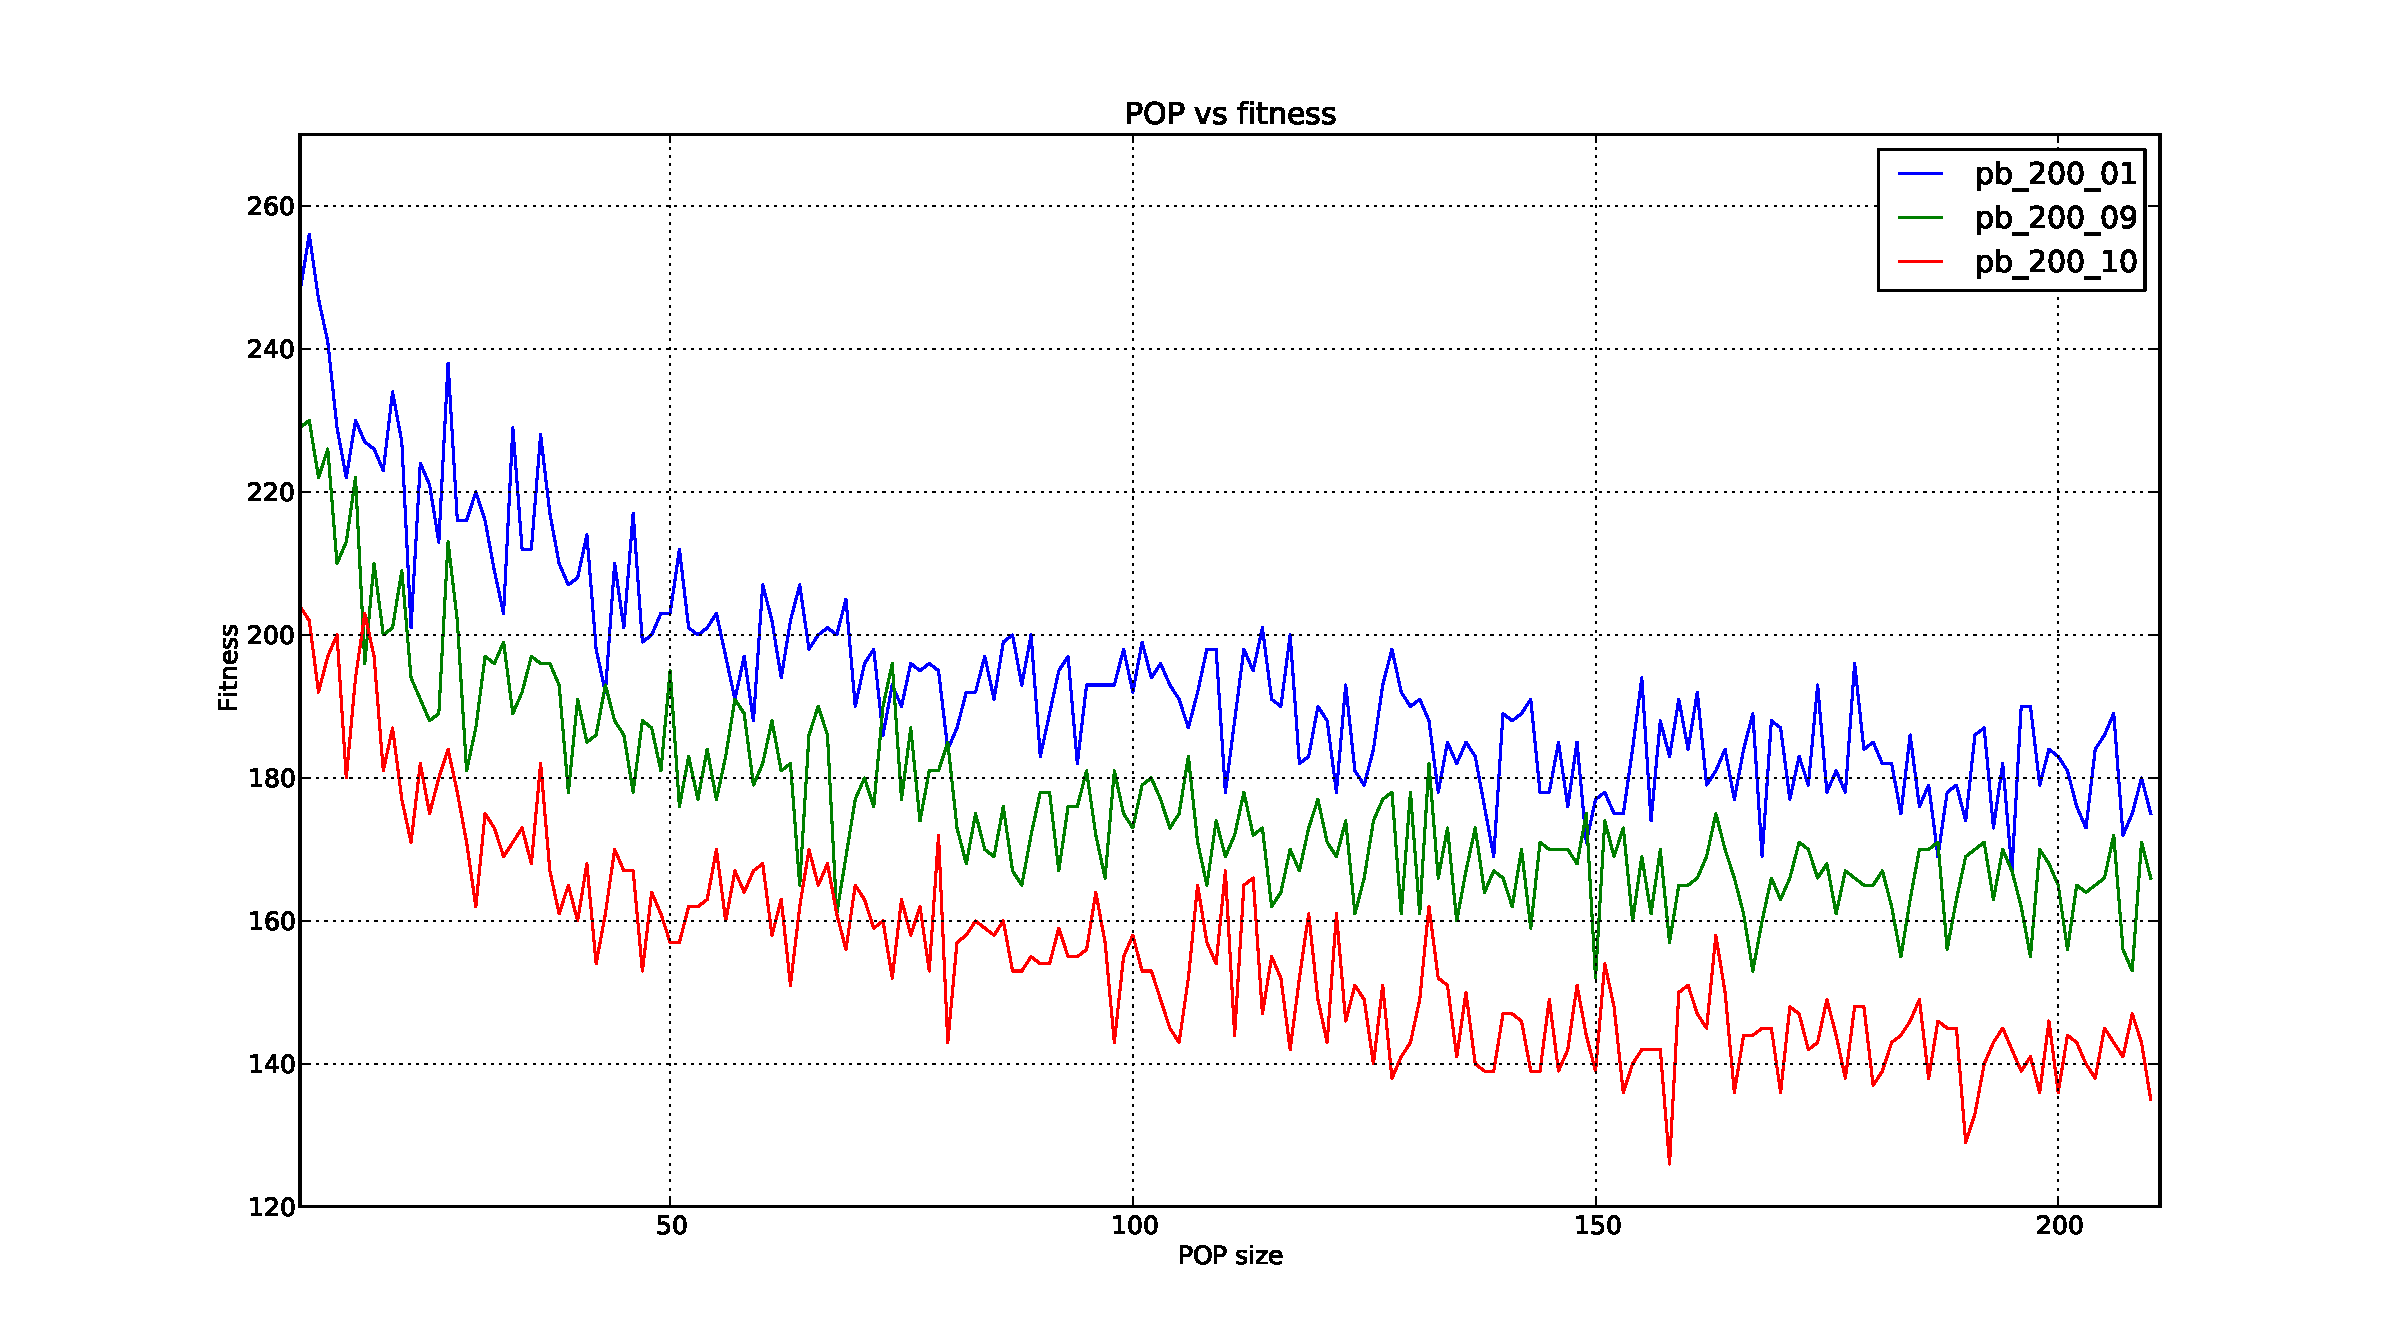
\includegraphics[width=0.95\textwidth]{img/1.pdf}
	\caption{Comparaci\'on de las tres instancias dado un cambio en la poblaci\'on}
	\label{fig:1}
\end{center}
\end{figure}

\textbf{Configuración escogida:}\\

La siguiente tabla, proporciona la información pertinente del mejor resultado obtenido,
de las $200$ iteraciones en las que consistió la presente prueba por cada instancia.

Gracias a la figura~\ref{fig:1}, podemos darnos cuenta del comportamiento que nuestro
algoritmo va teniendo a medida que vamos aumentando el tamaño de la población.

En un comienzo podemos ver el pésimo comportamiento que posee, pues como la cantidad de
la población es muy pequeña, los anticuerpos no van a poder variar mucho, ya que al
momento de clonar o introducir diversidad, no cumplen su objetivo principal, pues
como estos procedimiento van a depender netamente del tamaño de la población, no serán
del todo útiles.

Cabe señalar que en realidad el comportamiento que está tomando el algoritmo, es más
bien siempre trabajar con soluciones aleatorias, pues la hipermutación de los clones
está determianda por el índice de la población, por lo que el mayor individuo se mutará
muy poco, lo que llevará a obtener pocas mejoras en nuestros anticuerpos.


\begin{center}
\begin{tabular}{|l|c|c|c|c|}
	\hline
	\textbf{Instancia} & \textbf{POP} & \textbf{Mejor resultado} & \textbf{Tiempo [s] } & \textbf{Tiempo total [s] }\\\hline
	\texttt{pb\_200\_01.txt} & 195 & 167 & 15.110 & 1608.853 \\\hline 
	\texttt{pb\_200\_09.txt} & 150 & 152 & 11.243 & 1593.739 \\\hline
	\texttt{pb\_200\_10.txt} & 158 & 126 & 11.210 & 1662.580 \\\hline
\end{tabular}
\end{center}

Las iteraciones luego de un tamaño en la población sobre $100$ aproximadamente,
se comienzan a comportar de una forma más normalizada, y la pendiente de la curva que aproxima
al comportamiento del algoritmo, se vuelve cada vez menor, lo cual está representado en la tabla,
ya que claramente los mejores rendimientos por cada instancia están sobre una población de
tamaño $100$.

A pesar de lo distinta que son cada instancia, en nivel de complejidad, los tiempos que toman
cada una están bien parecidas, entre $11$ y $15$ segundos, por lo que no hay mayor diferencia.
\newpage
\subsubsection{Número de generaciones}

\textbf{Prueba}: \blue{prueba2}\\

\textbf{Parámetros involucrados:} Número de generaciones \texttt{(GENS)}.\\

\textbf{Objetivo:} Analizar el comportamiento de acuerdo a fitness y tiempo de ejecución del número de generaciones entre un rango de valores.\\

\textbf{Metodología:} Se probarán varios valores en el rango de valores del parámetro \blue{[10,2000]} (iterando de 30 en 30).\\

\textbf{Gráfico:}\\

\begin{figure}[h!]
\begin{center}
	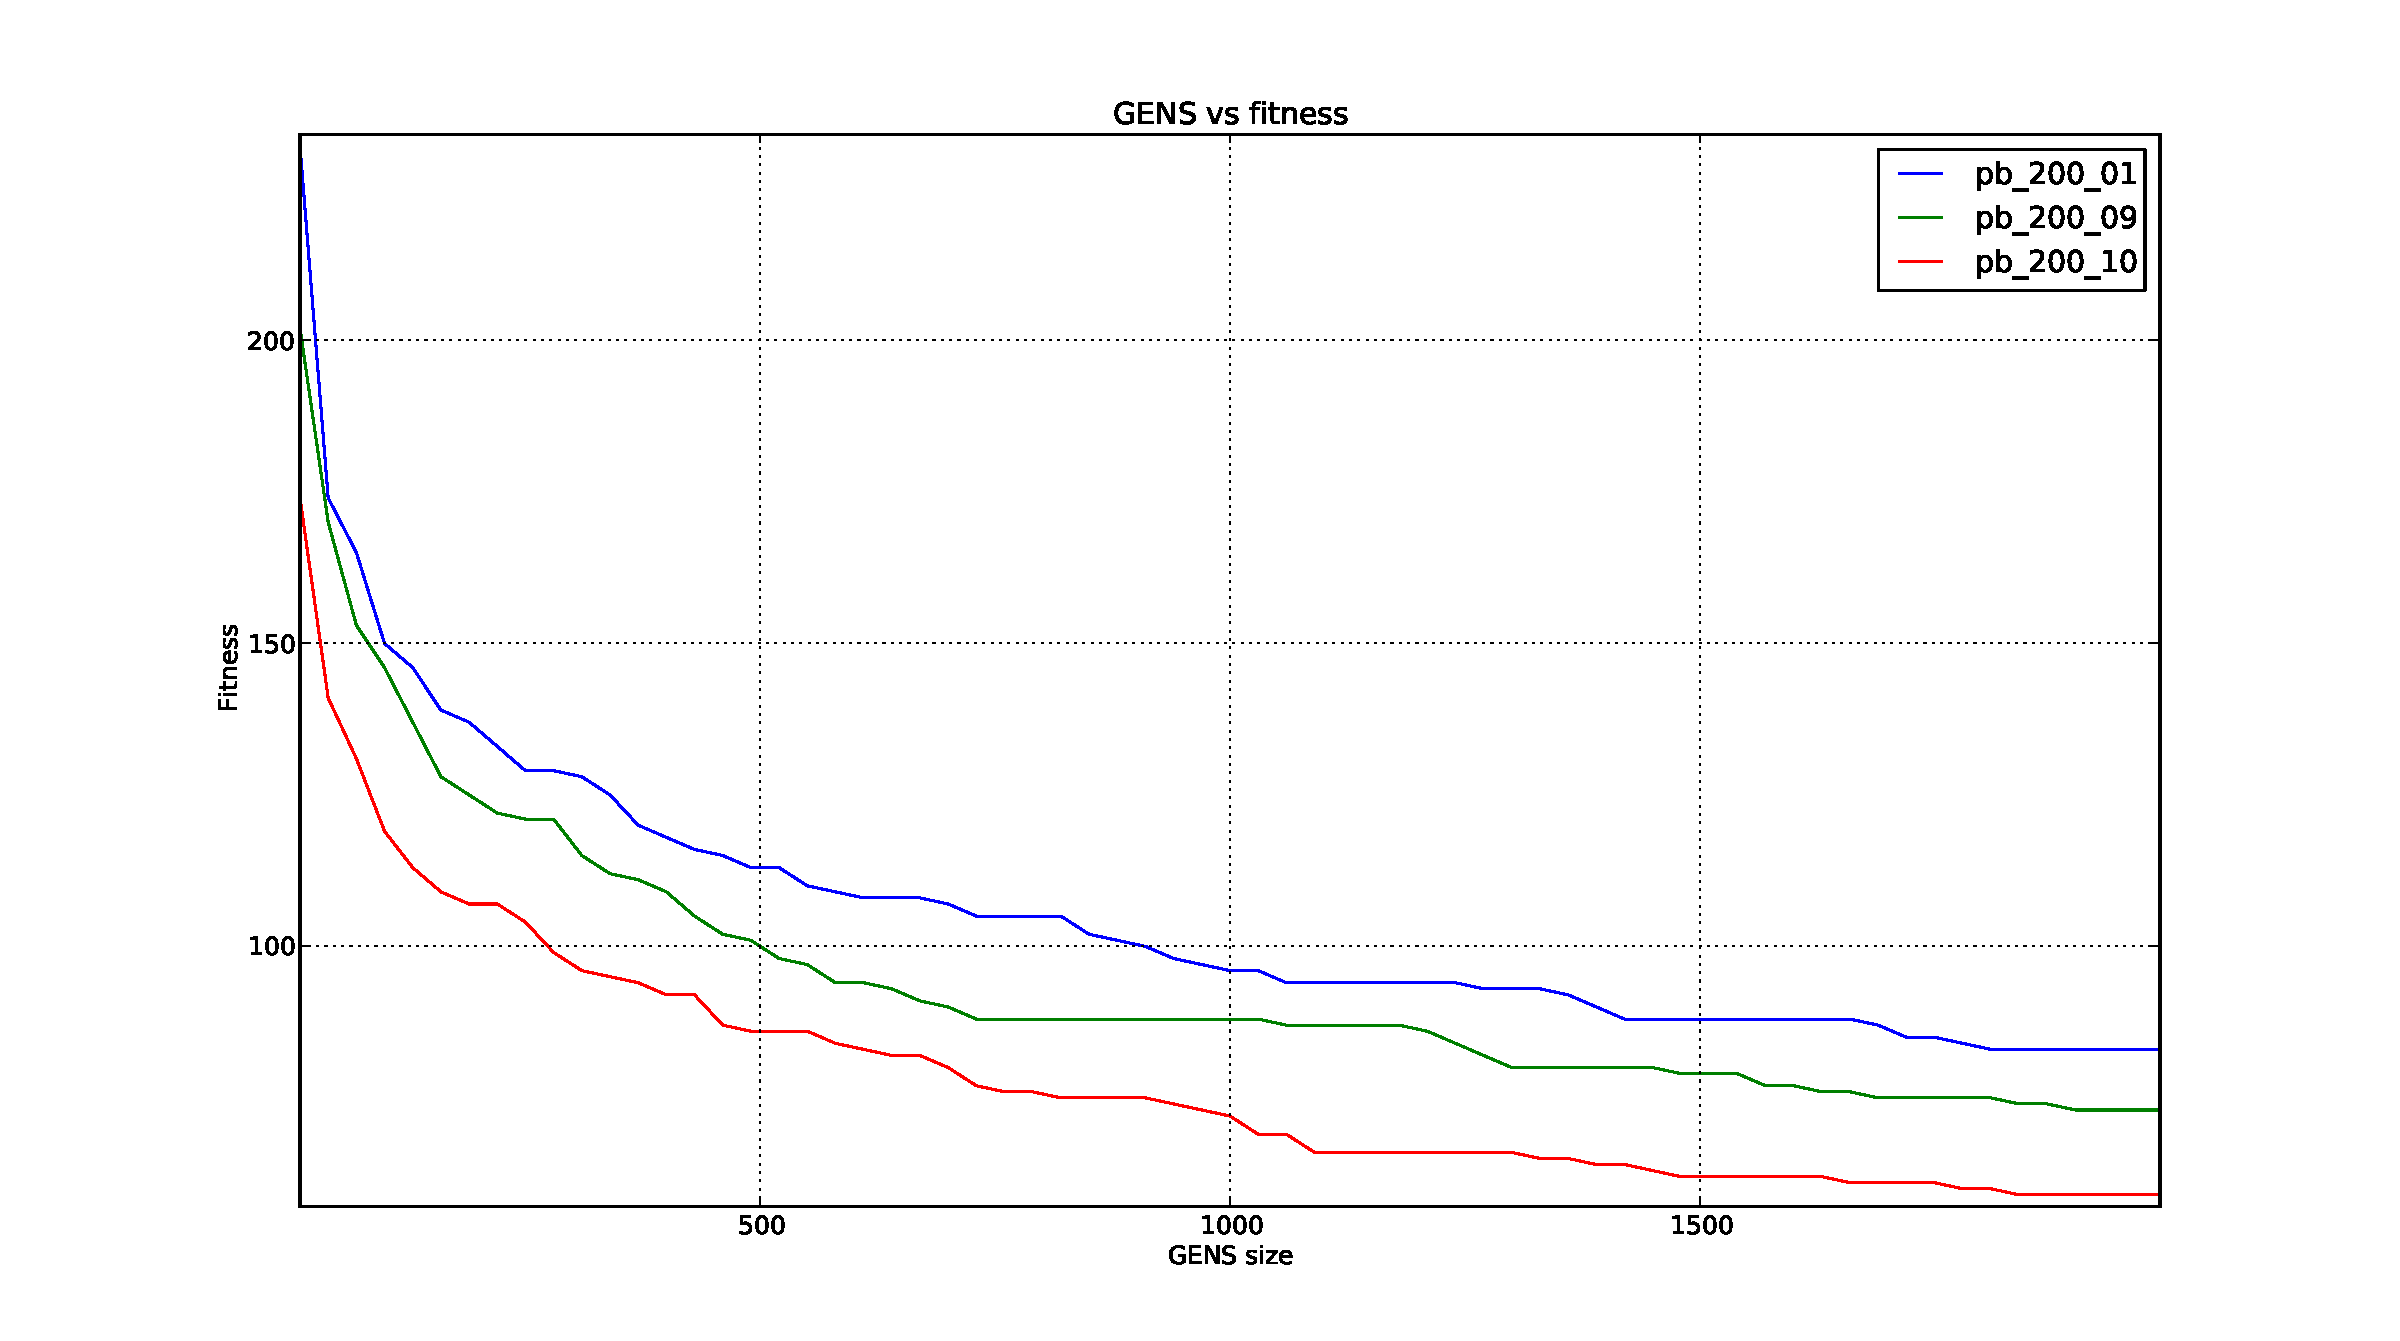
\includegraphics[width=0.95\textwidth]{img/2.pdf}
	\caption{Comparaci\'on de las tres instancias dado un cambio en el n\'umero de generaciones}
	\label{fig:2}
\end{center}
\end{figure}

\textbf{Configuración escogida:}\\

\begin{center}
\begin{tabular}{|l|c|c|c|c|}
	\hline
	\textbf{Instancia} & \textbf{GENS} &\textbf{Mejor resultado} & \textbf{Tiempo [s] } & \textbf{Tiempo total [s]}\\\hline
	\texttt{pb\_200\_01.txt} & 1810 & 186 & 7.782 & 256.177 \\\hline
	\texttt{pb\_200\_09.txt} & 1960 & 166 & 8.460 & 262.906 \\\hline
	\texttt{pb\_200\_10.txt} & 1630 & 144 & 7.562 & 256.546 \\\hline
\end{tabular}
\end{center}

\newpage
\subsubsection{Tasa de reemplazo}

\textbf{Prueba}: \blue{prueba3}\\

\textbf{Parámetros involucrados:} Tasa de reemplazo \texttt{(replaceRate)}.\\

\textbf{Objetivo:} Analizar el comportamiento de acuerdo a fitness y tiempo de ejecución de la tasa de reemplazo entre un rango de valores.\\

\textbf{Metodología:} Se probarán varios valores en el rango de valores del parámetro \blue{[0,1]}.
Para éste caso en particular, se ejecutó el algoritmo 10 veces por cada valor del parámetros y luego se seleccionó la mejor
para poder hacer el siguiente análisis.\\

\textbf{Gráfico:}\\

\begin{figure}[h!]
\begin{center}
	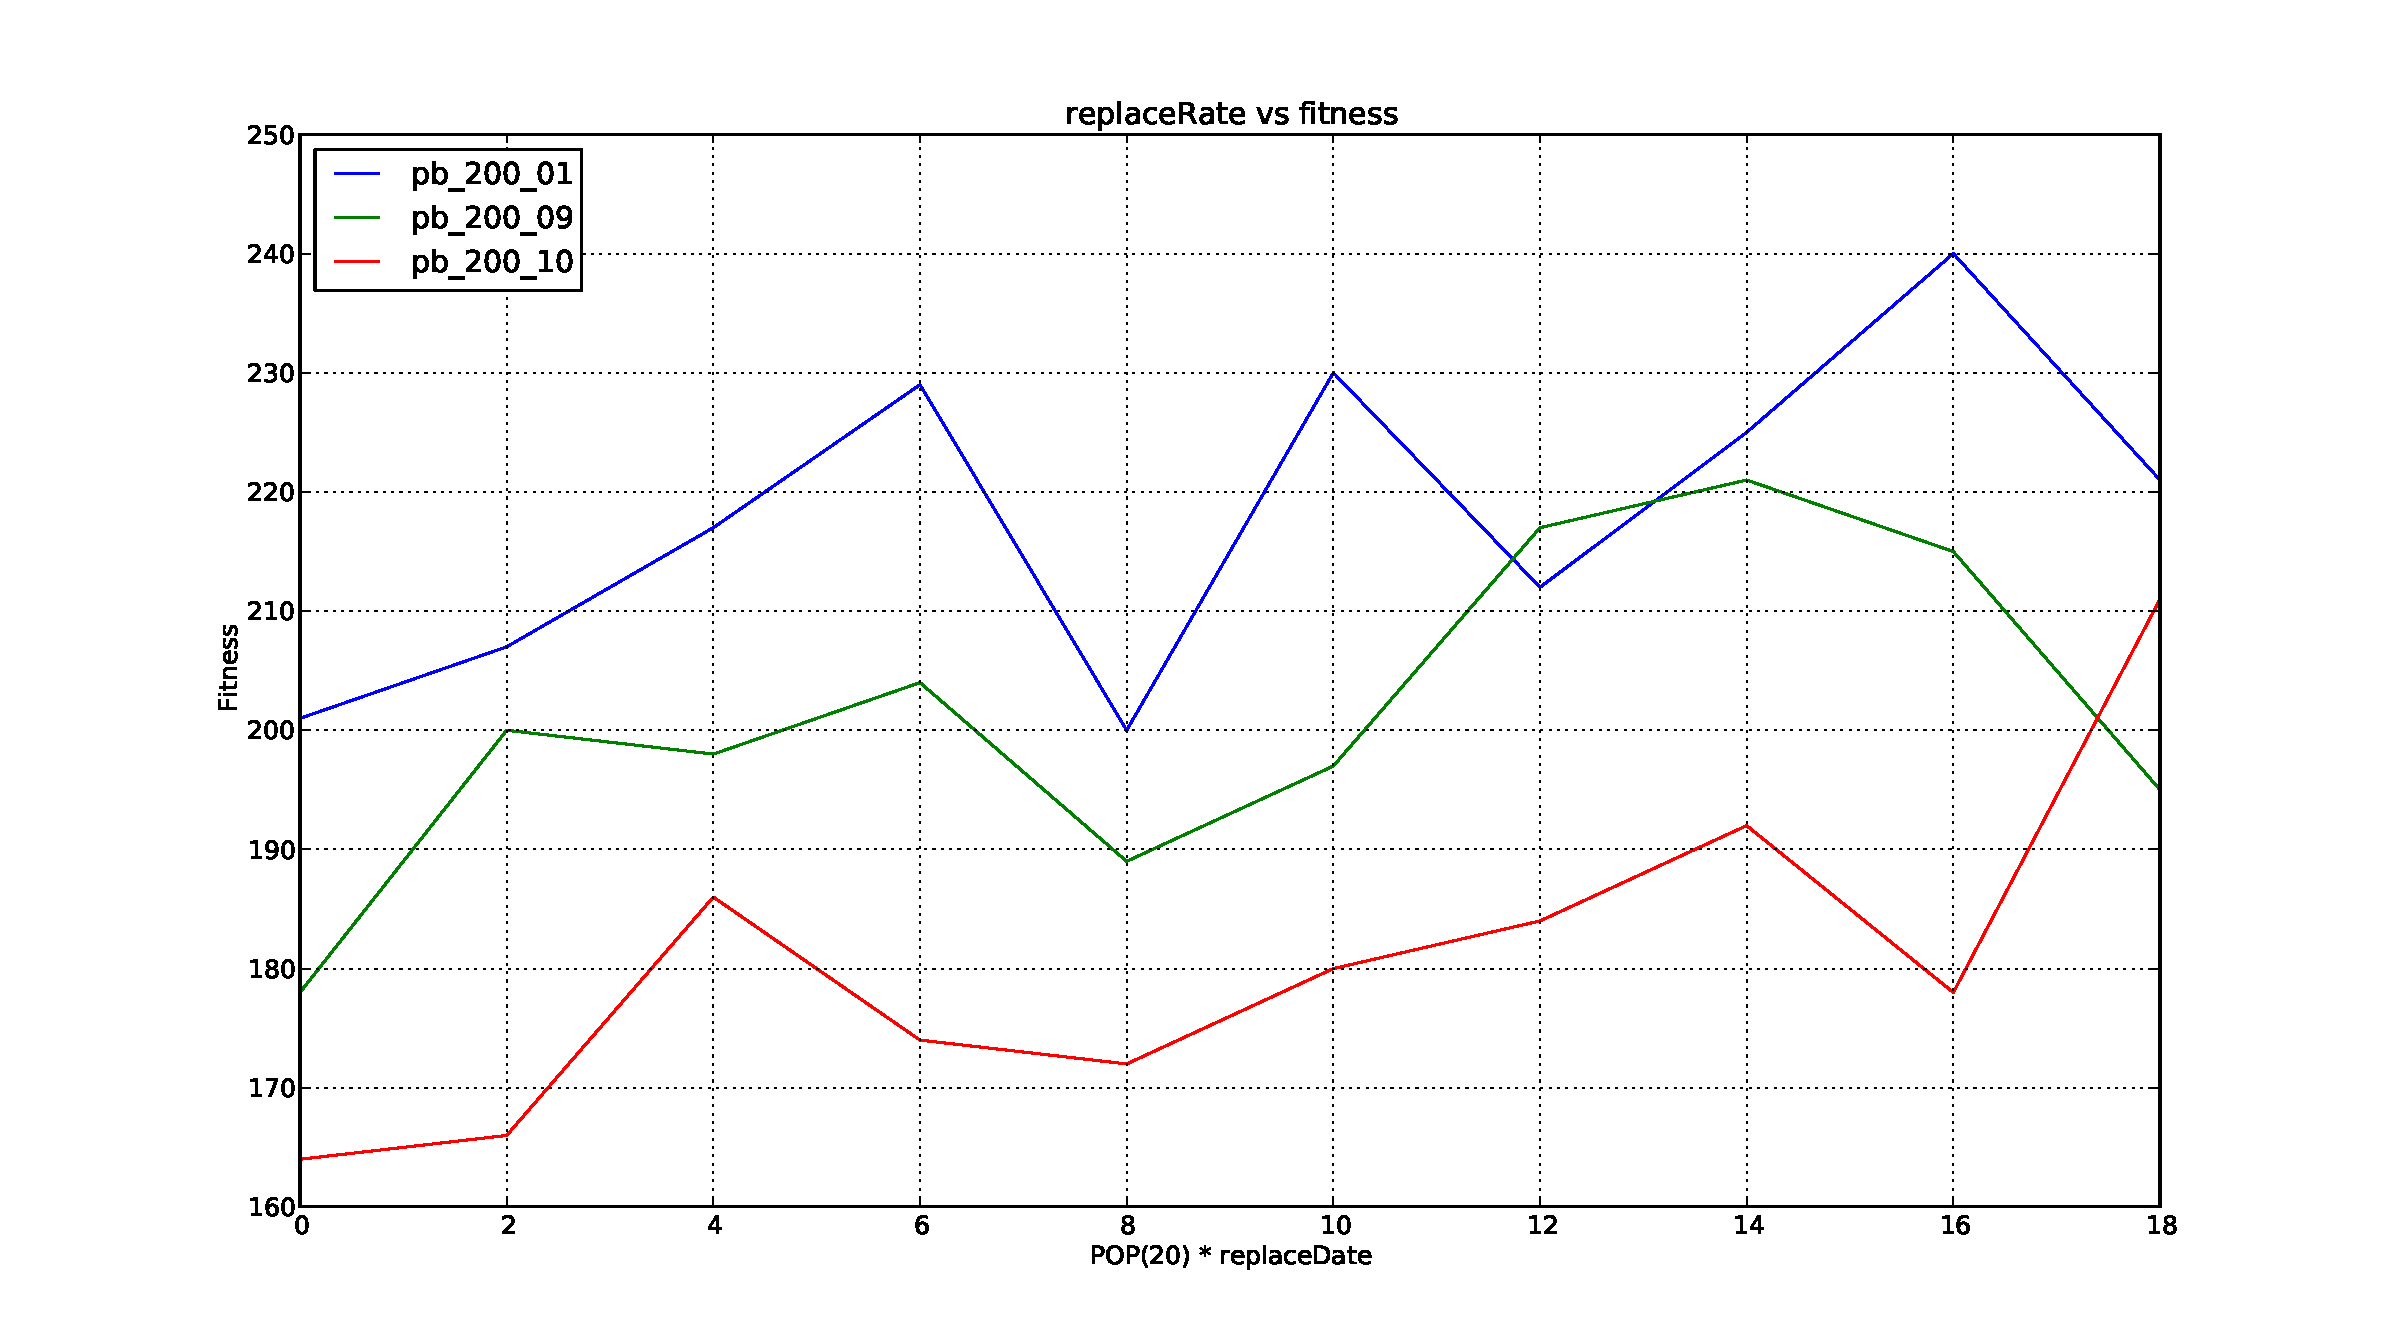
\includegraphics[width=0.95\textwidth]{img/3.pdf}
	\caption{Comparaci\'on de las tres instancias dado un cambio en la tasa de reemplazo}
	\label{fig:3}
\end{center}
\end{figure}

\textbf{Configuración escogida:}\\

La siguiente tabla, proporciona la información pertinente del mejor resultado obtenido,
de las $100$ iteraciones en las que consistió la presente prueba por cada instancia.

En éste caso, como se probaba la ``Tasa de reemplazo'' los valores posible son $0.1, 0.2, \ldots, 1.0$,
por lo que se realizó $10$ pruebas por cada valor.

Gracias a la figura~\ref{fig:3} nos podemos dar cuenta que los mejores valores se encuentran
para valores pequeños de la ``Tasa de reemplazo'' para las dos instancias finales, en cambio
para la primera instancia es un valor de $0.4$.

Podríamos ingenuamente decir, nuestro algoritmo no necesita ingresar diversidad y que por lo tanto
sólo nos dedicamos a \emph{explotar}, pero los resultados obtenidos se deben a que las iteraciones
que utilizamos como configuración básica son muy pocas, son sólo $200$, por lo que nuestro algoritmo
no alcanza a desarrollarse para poder tener la necesidad de salir de los ``óptimos locales'',
y así poder necesitar insertar diversidad, es por ésto que los valores de las dos últimas instancias,
es 0, pues el algoritmo no alcanza a necesitar diversidad.

\begin{center}
\begin{tabular}{|l|c|c|c|c|}
	\hline
	\textbf{Instancia} & \textbf{POP*replaceRate} & \textbf{Mejor resultado} & \textbf{Tiempo [s]} & \textbf{Tiempo total [s]}\\\hline
	\texttt{pb\_200\_01.txt} & 8 & 200 & 1.374 & 13.246 \\\hline
	\texttt{pb\_200\_09.txt} & 0 & 178 & 1.463 & 12.027 \\\hline
	\texttt{pb\_200\_10.txt} & 0 & 164 & 0.515 & 12.133   \\\hline
\end{tabular}
\end{center}


\newpage
\subsubsection{Factor de clonación y Tasa de clonación}

\textbf{Prueba}: \blue{prueba4} \\

\textbf{Parámetros involucrados}: Tasa de clonación y Factor de clonación. \\

\textbf{Objetivo}: Estudiar el efecto de la tasa y el factor de clonación en conjunto de acuerdo a fitness obtenido para la variación
de los dos parámetros en todo tu dominio.\\

\textbf{Metodología}: Se prueban varias combinaciones de valores para ver el efecto de los parámetros y poder observar su comportamiento.\\

\textbf{Configuración escogida:}\\

\begin{small}
\begin{center}
\begin{tabular}{|l|c|c|c|c|c|}
	\hline
	\textbf{Instancia} & \textbf{clonationRate} & \textbf{clonationFactor} &\textbf{Mejor resultado} & \textbf{Tiempo [s]} & \textbf{Tiempo total [s]}\\\hline
	\texttt{pb\_200\_01.txt} & 0.6 & 1   & 192 & 1.241 & 132.608 \\\hline
	\texttt{pb\_200\_09.txt} & 0.6 & 1   & 180 & 1.378 & 132.068 \\\hline
	\texttt{pb\_200\_10.txt} & 0.5 & 0.9 & 160 & 1.379 & 132.124 \\\hline
\end{tabular}
\end{center}
\end{small}
\normalsize
\textbf{Gráfico:}\\

\begin{figure}[h!]
\begin{center}
	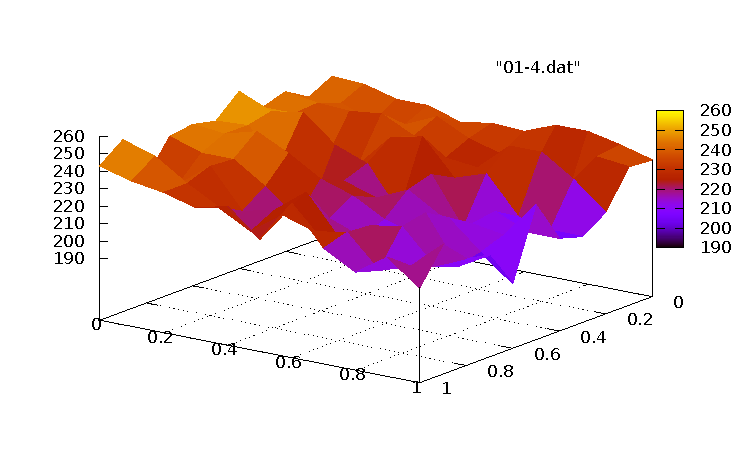
\includegraphics[width=0.95\textwidth]{img/01-4.pdf}
	\caption{Comparaci\'on de la instancia \texttt{pb\_200\_01.txt} variando \texttt{clonationRate} y \texttt{clonationFactor}}
	\label{fig:4-1}
\end{center}
\end{figure}

\begin{figure}[h!]
\begin{center}
	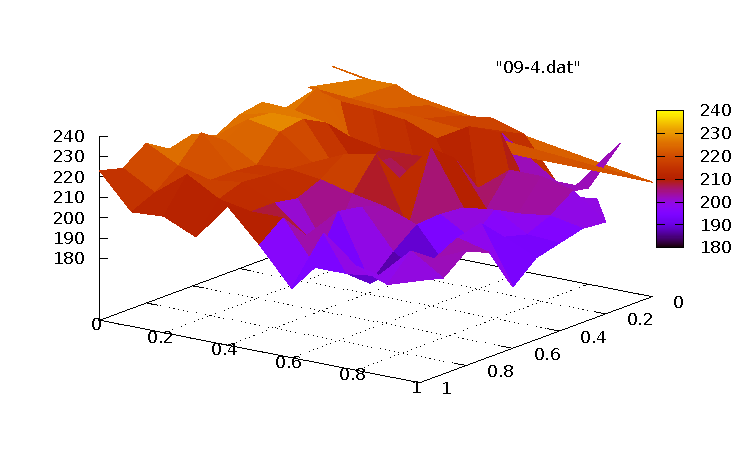
\includegraphics[width=0.95\textwidth]{img/09-4.pdf}
	\caption{Comparaci\'on de la instancia \texttt{pb\_200\_09.txt} variando \texttt{clonationRate} y \texttt{clonationFactor}}
	\label{fig:4-2}
\end{center}
\end{figure}

\newpage 
\begin{figure}[h!]
\begin{center}
	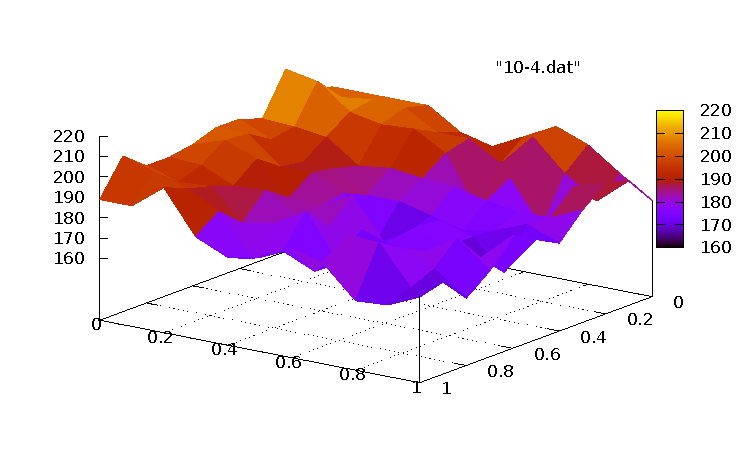
\includegraphics[width=0.95\textwidth]{img/10-4.pdf}
	\caption{Comparaci\'on de la instancia \texttt{pb\_200\_10.txt} variando \texttt{clonationRate} y \texttt{clonationFactor}}
	\label{fig:4-3}
\end{center}
\end{figure}


\newpage
%
%
%elegir una configuración para cada instancia
%	-indicar el fitness
%	-identificar claramente las características del algoritmo.
%	-estimación del tiempo en realizarla.

\subsubsection{Sintonización Automática}
\frame
{
\frametitle{Sintonización Automática}
\begin{itemize}
	\item 
\end{itemize}
}


\newpage
\section{Control de Parámetros}
\label{sec:control}
Antes de comenzar a describir y analizar los resultados del control efectuado,
es necesario poder conocer un poco el comportamiento del algoritmo.

Luego de la sintonización, se escogió la siguiente configuración para el problema:

\begin{itemize}
    \item \texttt{POP = 160}
    \item \texttt{GENS = 2000}
    \item \texttt{clonationFactor = 0.8}
    \item \texttt{clonationRate = 0.8}
    \item \texttt{replaceRate = 0.5}
\end{itemize}

Aparte de los cambios en la configuración básica, también el algoritmo fue modificado
en términos de normalizar el funcionamiento de la generación de números aleatorios,
pues anteriormente la generación de números aleatorios era completamente distinta en
cada ejecución del algoritmo, por lo que ahora se estableció una forma para la población
inicial y para caga iteración se va modificando la \emph{semilla} para generar
los anticuerpos de la fase de diversidad.

Teniendo en cuenta la configuración previa, se consideró importante centrar la atención
para hacer el control en dos aspectos. Primero se realizó una función para determinar
el \emph{promedio del fitness de una población} y otra función para determinar el
\emph{mejor fitness de una población}.

La razón para poder centrar la atención en esas dos funciones, es para poder
determinar si la nueva generación es mejor o peor en términos de \emph{fitness},
para que nos servirá el \emph{promedio}, por otro lado, al obtener al mejor individuo
podemos darnos cuenta si ha habido alguna mejora, ya que si es el mejor, se clonará
más veces en la siguiente iteración.

Por lo tanto los resultados obtenidos con la configuración inicial, con respecto a la
cantidad de veces en que la \textbf{diferencia} entre los \emph{promedios del fitness} y la \textbf{diferencia}
de los \emph{mejores fitness} fue positiva, cero o negativa:


\begin{center}
\begin{tabular}{|l|c|c|c|c|c|c|c|c|}
\hline
  & \multicolumn{3}{|c|}{\textbf{$\Delta$ promedios}} & \multicolumn{3}{|c|}{\textbf{$\Delta$ mejores}} & & \\\hline
\textbf{Instancia} & $+\Delta$ & $0$ & $-\Delta$ & $+\Delta$ & $0$ & $-\Delta$ & \textbf{Fitness} & \textbf{Tiempo} \\\hline
\texttt{pb\_200\_01.txt} & 0 & 0 & 2000 & 1624 & 289 & 87 & 77 & 104.451 \\\hline
\texttt{pb\_200\_09.txt} & 0 & 0 & 2000 & 1605 & 324 & 71 & 71 & 104.833 \\\hline
\texttt{pb\_200\_10.txt} & 0 & 0 & 2000 & 1442 & 486 & 72 & 55 & 102.377 \\\hline
\end{tabular}
\end{center}

La anterior tabla nos da a entender su comportamiento,
por ejemplo, el algoritmo está desarrollado de una forma que siempre
la diferencia del promedio de los  fitness de la nueva generación de clones,
con  el de la población actual será negativo, lo cual tiene una explicación
en que la población de clones son los mejores individuos de la población
y la hipermutación que se realiza no es mucha, como para crear individuos
muy distintos, por lo tanto siempre el promedio de la población actual será
mayor, es decir, más malo.

Por otro lado, para la diferencia entre el fitness de los mejores individuos,
tenemos que una gran cantidad de veces el comportamiento del algoritmo
indica que el mejor individuo de la población de clones es peor que
el mejor individuo de la población actual, lo cual se debe a la hipertmutación,
recordemos que como cada individuo se clona una determinada cantidad de veces,
pero tambien cada clon se muta, la mayoría de las veces el mejor individuo que
mutamos se vuelve peor de lo que era.

Pero tambien tenemos casos en que los mejores individuos son iguales
y otros en que el mejor individuo de la población de clones es mejor
que el de la población actual.

Para continuar con las implementaciones de control de parámetros,
tenemos los siguientes casos:
\newpage
\subsection{Primer Control}

La primera implementación no está basada en alguna publicación determinada,
si no que sigue la lógica de aumentar o disminuir la diversidad a medida
que tenemos mejores o peores individuos.

\begin{itemize}
\item \textbf{Parámetro a controlar:}
\begin{itemize}
	\item Tasa de reemplazo (\texttt{replaceRate}) \blue{[0,1]}.

	Éste parámetro va a determinar la cantidad de individuos que añadiremos a nuestra población,
	de manera que sean una fuente de diversidad y se obtiene multiplicando una probabilidad obtenida por
 el tamaño de la población
\end{itemize}
\item \textbf{Gatillador de cambio:} 
	En cada iteración se calculará la diferencia entre el \emph{fitness} de los mejores
	individuos, con la cual podremos tomar una determinada decisión.
	La diferencia se calcula de la forma:
	$$\text{Diferencia =  Mejor fitness de la población de clones - Mejor fitness de la población actual}$$
\item \textbf{Velocidad y mecanismo de cambio:} 
	A medida que calculamos la diferencia, vamos utilizando una variable que nos va indicando
	la cantidad de veces que ésta es positiva, cero o negativa.

	Para no realizar un cambio mínimo en cada iteración se estableció un valor de acumulación
	del $0.2\%$ del total de generaciones totales, para poder cambiar el valor de la tasa de reemplazo.

	Si la tasa es negativa, es decir si en la población de clones tenemos el mejor fitness, vamos a
	introducir menos diversidad a nuestra nueva población por lo que disminuimos la tasa de reemplazo,
	en una cantidad equivalente al $10\%$ de la población. Y para el caso contrario, se aumenta en la misma
	cantidad.
\newpage
\item \textbf{Pseudocódigo:} 
\begin{alltt}
    Inicio
    g <- 0 // numero de generaciones
    Leer datos de entrada
    Población <- Generar población inicial
    Evaluar población

    Mientras g < GENS
        Limpiar poblaciones
        \blue{Guardar mejor individuo de la población}
        Seleccionar individuos a clonal (ruleta)
        Clonación (fórmula)
        Hipermutación mediante Swap
        Evaluar población mutada
        Selección de clones (Mejores)
        \blue{Guardar mejor individuo de los clones
        Calcular diferencia entre mejores individuos
        Si diferencia < 0
            aumentar contadorA
            Si contador = 0.2\% GENS
               Tasa de reemplazo = Tasa de reemplazo - 10\% POP
               contadorA = 0
        O Sino diferencia > 0
            aumentar contadorB
            Si contadorB = 0.2\% GENS y Tasa de reemplazo < 90\%POP
               	Tasa de reemplazo = Tasa de reemplazo + 10\% POP
                contadorB = 0
        O Sino diferencia = 0
            Tasa de reemplazo = 50\% POP
            contadorA = 0
            contadorB = 0 
		}
        Inserción de clones en nueva población
        Generar elementos nuevos aleatorios
        Inserción de elementos nuevos al población
        g <- g + 1
    Fin Mientras

    Imprimir resultados
    Fin
\end{alltt}

\end{itemize}
\newpage
\subsection{Segundo Control}

La presente implementación se basa en la escencia de la técnica
mostrada por Riff et al~\cite{riff}, ya que debido a que la implementación
del algoritmo de selección clonal es distinta, pero se obtiene
la idea central implementada y cambiando el enfoque en el sentido
que en la publicación la función maximiza y la presente implementación
minimiza.

\begin{itemize}
\item \textbf{Parámetro a controlar:}
\begin{itemize}
	\item Control de clonación (\texttt{clonation\_control}) \blue{[-90\% POP, 90\% POP]}

		Factor que se le va a sumar a la cantidad de clones que generamos por cada
		individuo seleccionado. Éste factor puede tanto disminuir como aumentar la cantidad
		de clones de un individuo.		
	\item Tasa de clonacion (\texttt{clonationRate}) \blue{[0,1]}

		Parámetro que va a establecer la cantidad de individuos que pasan al proceso
		de clonación y se obtiene multiplicando una probabilidad obtenida por el tamaño de la población.

\end{itemize}
\item \textbf{Gatillador de cambio:} 

	En cada iteración se calculará la diferencia entre el \emph{fitness} de los mejores
	individuos, y la diferencia entre el promedio de los fittness de ambas poblaciones,
	con los cuales podremos tomar una determinada decisión.
	Las diferencias se calculan de la forma:
	$$\text{Diferencia Mejores =  Mejor fitness de la población de clones - Mejor fitness de la población actual}$$
	$$\text{Diferencia Promedio =  Promedio fitness de la población de clones - Promedio fitness de la población actual}$$

\item \textbf{Velocidad y mecanismo de cambio:}

	A medida que calculamos las diferencias, vamos tomando una decisión dependiendo si
	son positivas, cero o negativas.

	En cada condición, controlamos que el control de clonación no se escape de los rangos
	establecidos y de la misma forma, aumentarmos el control de clonación en una unidad si la diferencia
	entre los mejores fitness de las poblaciones es menor, o sea si obtenemos un peor resultado,
	y viceversa.
	
	Al aumentar el factor clonamos más cada elemento, lo que nos va a favorecer aumentando
	la probabilidad de tener mejores individuos.

	Por otro lado si la diferencia entre los mejores individuos es negativa y la diferencia
	de los promedios es mayor, comenzamos a disminuir la tasa de clonación, para así
	comentar a seleccionar menos pues estamos ya con buenos resultados. También se tiene
	consideración para controlar la tasa de clonación, puesto que por ejemeplo seleccionar
	sólo un individuo para clonar no tiene sentido.
\newpage
\item \textbf{Pseudocódigo:} 

\begin{alltt}
    Inicio
    g <- 0 // numero de generaciones
	control clonacion <- 0 
    Leer datos de entrada
    Población <- Generar población inicial
    Evaluar población

    Mientras g < GENS
        Limpiar poblaciones
        \blue{Obtener mejor individuo de la población
        Obtener el promedio de los fitness de la población}
        Seleccionar individuos a clonal (ruleta)
        Clonación (fórmula)
        Hipermutación mediante Swap
        Evaluar población mutada
        Selección de clones (Mejores)
        \blue{Obtener mejor individuo de los clones
        Obtener el promedio de los fitness de los clones
        Calcular diferencia1 entre mejores individuos
        Calcular diferencia2 entre los promedios

        Si diferencia1 < 0 y control clonacion < 10\% POP
            control clonacion ++ 
        O Sino diferencia1 > 0 y control  clonacion > - 10\% POP
            control clonacion --

        Si diferencia1 < 0 y diferencia2 > 0 y Tasa de clonacion > 2
            Tasa de clonacion --
        O Sino Tasa de clonacion < 90\% POP
            Tasa de clonacion ++
		}
        Inserción de clones en nueva población
        Generar elementos nuevos aleatorios
        Inserción de elementos nuevos al población
        g <- g + 1
    Fin Mientras

    Imprimir resultados
    Fin
\end{alltt}
\end{itemize}


\newpage
\subsection{Resultados Control}
%Deberá realizar pruebas que comparen su algoritmo con y sin control, para eésto mantenga en ambos algoritmos los parámetros no controlados en un valor que usted considere bueno (utilizando la sección anterior), en el algoritmo sin control setee los parámetros elegidos para el control con los mejores valores encontrados. Compare los resultados en terminos de fitness y tiempo. 

\begin{center}
\begin{tabular}{|l|c|c|c|c|c|c|}
\hline
 & \multicolumn{2}{|c|}{Sin Control} & \multicolumn{2}{|c|}{1er Control} & \multicolumn{2}{|c|}{2do Control} \\\hline
\textbf{Instancias} & \textbf{Fitness} & \textbf{Tiempo} & \textbf{Fitness} & \textbf{Tiempo} & \textbf{Fitness} & \textbf{Tiempo} \\\hline
\texttt{pb\_200\_01.txt} & 77 & 104.734 & \red{75} & 101.152 & 76 & 105.692 \\ \hline
\texttt{pb\_200\_09.txt} & 71 & 104.156 & 66 & 102.252 & \red{64} & 104.641 \\ \hline
\texttt{pb\_200\_10.txt} & \red{55} & 103.314 & 63 & 102.146 & 63 & 105.684 \\ \hline
\end{tabular}
\end{center}

Si nos damos cuenta de los resultados obtenidos,
los dos mecanismos implementados no fueron 100\% útiles,
ya que las mejoras son casi insignificantes.
Ésto se puede deber a que falta un control sobre el resto de los parámetros
del algoritmo o simplemente que la forma en la cual se desarrolla el algoritmo
de selección clonal en sí, no es la más óptima, pues considerando la implementación
de Riff et al.~\cite{riff}, se seleccionan subconjuntos de las poblaciones para
poder calcular las diferencias de los promedios y de los mejores individuos.

Los mejores valores encontrados se encuentran dentro de las tres categorías,
por lo que no hay una preferencia determinada y lo mismo ocurre con el tiempo,
pues la implementación de control era demasiado simple como para añadir
un gran tiempo al total de tiempo de ejecución del algoritmo.


\newpage
\section{Resultados Generales}
\label{sec:resultados}
%El analisis de los datos obtenidos,
%	arrojara resultados que uds. deberan presentar en esta seccion.
%	Deben poner enfasis a los impactos del tema tecnologico en el
%	publico objetivo, y sus proyecciones.

En la sección anterior, pudimos darnos cuentas de los resultados de la encuesta realizada a personas que trabajan
en el mismo ambiente que se presenta en el trabajo, dándonos cuenta cuales herramientas utilizaban, si les eran útiles, etc,
pero ahora nos queremos enfocar en los \emph{impactos} principalmente, de nuestro tema principal, en el las personas estudiadas.

Con respecto a las tecnologías, podemos profundizar mucho acerca del proceso de \emph{selección}, \emph{desarrollo} y su propio \emph{uso},
y sobre todo, en el análisis a los impactos producidos por cada uno de los factores anteriormente señalados.
Éstos impactos, no influyen sólo en la persona, sino que van más allá, poseen una suerte de influencia en el quehacer humano y por ende
todo lo que lo rodea, \emph{alterando} su comportamiento.

Analizando uno de los investigadores más importantes en ésta área, McLuhan~\cite{mcluhan}, podemos obtener ciertas preguntas que nos van a servir para ver el impacto
de las tecnologías en nuestro ambiente.
Las preguntas son:
\begin{itemize}
	\item ¿Qué genera, crea o posibilita?
	\item ¿Qué preserva o aumenta?
 	\item ¿Qué recupera o revaloriza?
	\item ¿Qué reemplaza o deja obsoleto?
\end{itemize}

Las cuales debemos resolver por cada tecnología que se quiera evaluar.

Si consideramos las \emph{tecnologías de la información} como un elemento tecnológico, podemos pasar a responder dichas preguntas para el trabajo en general:
\begin{itemize}
	\item \emph{¿Qué genera, crea o posibilita?}\\
		Gracias a las tecnologías de la información, estamos generando nuevos caminos de comunicación para realizar determinadas actividades en cualquier área,
		creando así las instancias necesarias, para que la comunicación sea bastante directa, en comparación a metodologías antiguas.
		
		Tomando en cuenta lo anterior estamos posibilitando, que dos o más personas en lugares totalmente distintos en el mundo, puedan trabajar en conjunto,
		sin tener la necesidad de una cercanía física, lo cual nos sirve para obtener una especie de comodidad a la hora de trabajar.
		
	\item \emph{¿Qué preserva o aumenta?}\\
		Estamos preservando y aumentando en algunos casos, la cantidad de trabajo realizado en conjunto, pues tenemos que tener en cuenta que al existir una
		comunicación más fluida, aumentamos la relación de dos distintas organizaciones, en un proyecto determinado.

		Por otra parte, aumenta la capacidad de que grupos pequeños de estudiantes con una misma motivación, puedan realizar actividades que contribuyan
		a proyectos mundiales, en los cuales por una razón económica, o quizás considerando la comodidad, no pueden estar presentes en un determinado lugar
		en el mundo.
	
		Tomando en cuenta ambos puntos, podemos darnos cuenta, que el crecimiento como profesional de un determinado estudiante, crece enormemente,
		pues ya no está sometido a un estilo de trabajo local, de su universidad y/o entorno, conociendo nuevas costumbres, estilos de trabajo, etc.

 	\item \emph{¿Qué recupera o revaloriza?}\\
		Al momento de abastecernos con todas los recursos necesarios utilizando tecnologías de la información, podemos comenzar a recuperar valores o 
		buenas costumbres al momento de realizar un proyecto, revalorizando el trabajo realizado; con ésto nos referimos a que cuando uno se encuentra
		en un establecimiento educacional y realiza cierto proyecto, no tiene el mismo valor, obtener una buena calificación en una asignatura determinada,
		que se reconozca el mismo trabajo, por una organización mundialmente conocida.

		Comenzamos a darnos cuenta, que junto a la perseverancia podemos llegar a cumplir objetivos bastante ambiciosos.		

	\item \emph{¿Qué reemplaza o deja obsoleto?}\\
		Si el uso de la tecnología no es utilizado de una buena forma, es decir, no abusando y llevando al máximo las comodidades que nos ofrece,
		se puede transformar en algo negativo para una persona o un entorno social, reemplazando todo lo que son las relaciones interpersonales,
		el poder entablar una conversación ``en persona'' con algún otro individuo.

		Por otro lado, la tecnología actual ha dejado de lado (no del todo) a medios de comunicación antiguos, como lo son las cartas tradicionales,
		el Fax, el telégrafo, etc , que en su tiempo, fueron lo último de la tecnología, con lo que podemos decir, que la misma tecnología,
		deja obsoleta a la tecnología.

\end{itemize}

Considerando que éste análisis puedo no ser del todo completo con respecto a la apreciación de los impactos de las \emph{tecnologías de la información},
existen trabajos complementarios para comprender mucho mejor los fenómenos observados.

Para identificar mejor los impactos, ya sean negativos o positivos de las distintas actividades relacionadas con tecnologías sobre las personas,
Solivérez~\cite{soliverez} propone un nuevo conjunto de preguntas:
\begin{itemize}
	\item \emph{Impacto práctico:}
	\begin{itemize}
		\item ¿Para qué sirve?
		\item ¿Qué permite hacer que sin ella sería imposible?
		\item ¿Qué facilita?
	\end{itemize}
	\item \emph{Impacto simbólico:}
	\begin{itemize}
		\item ¿Qué simboliza o representa?
		\item ¿Qué connota?
	\end{itemize}
	\item \emph{Impacto tecnológico:}
	\begin{itemize}
		\item ¿Qué objetos o saberes técnicos preexistentes lo hacen posible?
		\item ¿Qué reemplaza o deja obsoleto?
		\item ¿Qué disminuye o hace menos probable?
		\item ¿Qué recupera o revaloriza?
		\item ¿Qué obstáculos al desarrollo de otras tecnologías elimina?
	\end{itemize}
	\item \emph{Impacto ambiental:}
	\begin{itemize}
		\item ¿El uso de qué recursos aumenta, disminuye o reemplaza?
		\item ¿Qué residuos o emanaciones produce?
		\item ¿Qué efectos tiene sobre la vida animal y vegetal?
	\end{itemize}
	\item \emph{Impacto ético:}
	\begin{itemize}
		\item ¿Qué necesidad humana básica permite satisfacer mejor?
		\item ¿Qué deseos genera o potencia?
		\item ¿Qué daños reversibles o irreversibles causa?
		\item ¿Qué alternativas más beneficiosas existen?
	\end{itemize}
	\item \emph{Impacto epistemológico:}
	\begin{itemize}
		\item ¿Qué conocimientos previos cuestiona?
		\item ¿Qué nuevos campos de conocimiento abre o potencia?
	\end{itemize}
\end{itemize}

Las cuales nos van a permitir obtener un argumento mas completo a la hora de analizar los impactos que nos interesan.
Para éste caso sólo nos limitaremos a analizar el \emph{Impacto Ético}.

\begin{itemize}
	\item \emph{¿Qué necesidad humana básica permite satisfacer mejor?}\\
		La necesidad de la comunicación con personas que no se encuentres cerca, geográficamente hablando.
		Estamos mucho más conectados con todo el mundo, por lo que no importa el lugar, siempre podremos
		estar en contacto de las personas que necesitemos.

	\item \emph{¿Qué deseos genera o potencia?}\\
		Los deseos de continuar con distintos proyectos, en nuevas organizaciones, generar grupos de trabajo,
		potenciando el trabajo en equipo internacional, lo cual se ve beneficiado al momento de querer
		generar lazos aún más fuertes, donde se recurren a eventos como \emph{Workshops} en algún lugar del mundo,
		donde aparte de conocer a las personas e interactuar con ellas, se crean nuevos lazos que podrán estar
		vigentes con el pasar del tiempo, gracias a la tecnología de la información.

	\item \emph{¿Qué daños reversibles o irreversibles causa?}\\
		Con respecto a los daños reversibles, tenemos la adicción a la información que se ha dado en varias personas,
		tomando las palabras del último trabajo del ramo, puede producirse una esclavitud tecnológica.
		Por otro lado tenemos el problema anteriormente señalado, que es la pérdida de las relaciones sociales,
		que puede ser controlada, moderando el uso de los medios de comunicación tecnológicos actuales.

		Ahora considerando los daños irreversibles, tenemos que la actitud de algunas personas puede transformarse
		negativamente a asumir la facilidad de obtener o realizar tareas, sin ir más lejos los daños al lenguaje,
		que hoy en día la juventud posee, que tienen como fin sólo agilizar la comunicación, alterando el mensaje.
		
		Pero concentrándonos en nuestro problema, el único problema que se puede temer,
		son la pérdida de las relaciones interpersonales, que si bien es cierto considerando las colaboraciones
		internacionales es positivo que la gente trabaje, no hay que producir cierta esclavitud, no podemos vivir
		sin relacionarnos con otras personas, ya que eso es lo que sustenta la sociedad.

	\item \emph{¿Qué alternativas más beneficiosas existen?}\\
		Más que buscar una alternativa a las tecnologías de la información, tenemos el fiel pensamiento de que
		no hay que buscar alternativas sino que hay que aprender a vivir con la tecnología, que hoy por hoy,
		nadie sabe utilizar de la mejor forma la tecnología.

		¿Tenemos clara la noción de lo bueno y lo malo? a veces la información puede alterar nuestra percepción
		de ciertas actividades, pero en el caso de las relaciones internacionales, no se ve tanta coherencia
		a la presente idea.
\end{itemize}


\newpage
\section{Conclusiones}
\label{sec:conclusiones}
%De acuerdo a la introducci\'on que se hizo, entregar afirmaciones
%  basadas en los experimientos y sus resultados.

A primera vista, los resultados obtenidos en la presente implementación, superan en gran medida a los óptimos encontrados
en todos estos años, donde distintas personas, han utilizado, variadas técnicas para poder resolver el \emph{Car Sequencing Problem}
de la mejor manera, considerando así, que se pudieron haber utilizado técnicas completas, que si bien es cierto, pueden demorar mucho,
van a encontrar el \emph{óptimo global} de un determinado problema, lo cual se diferencia notoriamente con las técnicas incompletas,
como es el caso de ka presente implementación, donde sólo se puede encontrar un \emph{óptimo local}.

Al mirar el gráfico podemos darnos cuenta, de que la distribución de la cantidad de restricciones violadas, poseen un comportamiento
bastante similar, guardando las proporciones de la cantidad de violaciones, lo que nos hace deducir, de que sólo nos falta un poco
más de control y sintonización de los parámetros utilizados, para acercarnos aún más a soluciones más óptimas.

Siguiendo con el análisis de los experimentos, podemos darnos cuenta de que si bien es cierto, las soluciones violan una cantidad
considerable de restricciones, estamos sacrificando una buena solución, por un corto tiempo de ejecución, el cual en algunos casos,
sólo llega a durar 1 minuto, lo que comparado con el tiempo de alguna técnica completa, que puede durar días, nos beneficia de cierta manera.

Con respecto a la representación del problema, existen ciertos pros y contras.
Primero que todo la representación que se utilizó en la presente implementación,
consiste en una del tipo no-binaría, por lo que no es tan fácil utilizar los típicos movimientos de las representaciones binarias,
como lo son el \emph{bit-flip} y el \emph{cruzamiento en un punto}, ya que estaríamos violando las restricciones duras del problema,
por lo cual en la presente implementación, por ejemplo, no se utilizó un operador de cruzamiento y sólo se deposito la confianza,
en la mutación con \emph{Simulated Annealing} que se encargó tanto de explorar como de explotar.

Según lo anteriormente dicho, el no poseer un operador de cruzamiento, puede haber perjudicado la explotación del presente algoritmo
evolutivo, y por ende, entorpecido la búsqueda de un óptimo local. Aunque los resultados no fueron del todo malos, por lo que el simulated annealing
hizo su trabajo explorando y explotando, pero no de la forma más apropiada.

Otro punto importante en la presente implementación, es la forma en la cual se genera la población inicial.
Como ya hemos mencionado anteriormente, lo favorable del método utilizado es que se generan soluciones factibles,
es decir, que cumplen las restricciones duras, pero por otro lado, éstas se generan de forma aleatoria, lo cual indica,
que quizás utilizando alguna técnica de construcción de individuos más apropiada, como Greedy o GRASP, la calidad de la
población inicial aumentaría, lo cual sería interesante como trabajo futuro.


Con respecto a la mutación con simulated annealing, cabe señalar que existen algunos aspectos que pueden ser mejorados,
como por ejemplo un control de la temperatura, pues en la presente implementación, la temperatura disminuye cada 3 iteraciones,
lo que si tomamos en cuenta un control más riguroso, como comparar la calidad de las soluciones generadas, podríamos
realizar los cambios en la temperatura, a medida que el algoritmo se comporta de una forma más apropiada.


Finalmente, es posible mejorar la presente implementación de un algoritmo evolutivo aumentando la exploración,
que en éste caso significa poder mejorar lo que es la mutación, ya que dentro del simulated annealing, el movimiento
no es muy apropiado, y quizás el sólo hecho de mejorar el movimiento de la mutación simulated annealing, puede
traer un mejor desempeño en nuestro algoritmo. Otra forma podría ser cambiar el método de la ruleta, pues si bien es cierto,
le entrega una mayor probabilidad para escoger los mejores individuos, no nos prohibe elegir malos individuos, lo que
perjudica a nuestra siguiente población, y por ende a la solución del problema.


% OLD

%Conclusiones revelantes del estudio realizado.

%En el presente informe se ha dado un estado del arte de un problema muy popular
%en el área de la inteligencia artificial, el \emph{Car Sequencing Problem}, siendo éste
%una variación de otro problema connotado llamado \emph{Job Shop Scheduling}.
%Es tanto la importancia del presente problema, que la \emph{French Society of Operations
%Research and Decision-Making Aid} ha decidido ya hace varios años, comenzar lo que se denomina
%\emph{The ROADEF challenge} cada dos años, teniendo como objetivo central,  permitir a las personas
%que se desarrollan en el área de la industria el presenciar todos los avances y evoluciones
%en el ámbito de la Investigación de Operaciones y Análisis de Decisiones, pero no sólo eso
%sino el poder enfrentar directamente problemas decisionales complejos, que ocurren en la industria.
%Siguiendo la idea anterior, lo importante de éste \emph{Challenge} es que en el 2005, se consideró
%como tema principal el \emph{Car Sequencing Problem} debido a la propuesta que realizó RENAULT,
%por lo cual uno podrá imaginar la cantidad de avances que se produjeron, pues cada participante
%abordaba el problema desde una metodología distinta.
%
%Por otra parte, pareciera que un problema relacionado a \emph{ordenar} un conjunto de vehículos
%para ser ensamblados y así obtener el orden más óptimo, no es una tarea difícil, pero claramente
%debido a la complejidad que otorgan las restricciones y de que es un problema de la vida real,
%presenta un grado de dificultad mayor, lo cual queda reflejado por la cantidad de publicaciones 
%e investigaciones que hay al respecto.
%
%Se dieron a conocer también, tres áreas para atacar el presente problema.
%Por un lado tenemos los métodos heurísticos que como bien sabemos, es prácticamente jugar a la ruleta
%rusa con nuestra investigación, pues la heurística solamente selecciona un objetivo de los dos provenientes
%de la definición, una buena solución o un buen tiempo de ejecución. Pero también se presenta que la heurística
%es un mecanismo confiable para decidir \emph{utilizarlo} como un apoyo, mas que utilizarlo solo.
%
%Siguiendo con los mecanismos planteados, se vieron también los  métodos exactos,
%es decir, técnicas de optimización, donde podemos encontrar la \emph{programación lineal entera},
%\emph{branch and bound} y \emph{local search}, los cuales se dedicaban netamente a construir una
%solución óptima a partir de los datos que el mismo problema nos entrega. El único problema que tienen
%éstas técnicas es que la complejidad temporal va a crecer demasiado con respecto al tamaño de nuestro
%\emph{input} del algoritmo.
%
%Dentro de toda la lectura realizada para las distintas técnicas, pude percatarme que las mejores soluciones
%siempre son variaciones de métodos o tomar dos técnicas como complementarias, por ejemplo uno de los
%mejores resultados fue la combinación de un \emph{Ant Colony Optimization} con una heurística dinámica,
%pues claramente se nos señala que el buen uso de una heurística es crucial, es decir, hay que preocuparse
%de leer los estudios que se han publicado, par ver cual es la combinación más óptima.
%
%Finalmente, es impresionante la cantidad de estudios con respecto a éste problema en particular,
%por lo que podemos darnos cuenta que muchos centros de investigación han dedicado tiempo valioso
%para la resolución óptima del \emph{Car Sequencing Problem}, pero no tanto la versión que se estudió,
%que es la propuesta por Parello~\cite{parello}, sino mas bien al desafío de la ROADEF.


\newpage
\section{Bibliografía}
\bibliography{informe_final}

\newpage
\section{Anexo}
\label{sec:anexo}
\begin{tiny}
\lstinputlisting[language=Python]{dp.py}
\end{tiny}


\end{document} 
